\chapter{Stops}
The Turing-Welchman Bombe was remarkably adept at computing daily
keys in a tractable manner. In optimal conditions,
with a well-crafted and fortunate menu, the Bombe could run in as
little as 20 minutes and produce exactly the daily key needed to
decrypt messages.
To approach these optimal conditions, we must consider what it means
for one menu to be stronger than another. In this chapter, we will
explore the relationship
between menus and the number of stops the Bombe is expected to
encounter. Equipped with this information, a cryptanalyst would be
able to select the menu
that yields the fewest stops. Each stop consumed precious
time as operators needed to verify whether they corresponded to a
valid key. Therefore, menu selection becomes an integral factor
in reducing the time between intercepting transmissions and
recovering the key for that day. Even a reduction of minutes could
provide the slight edge that the Allies needed to preempt an attack.
Thus, developing an accurate model by which we can correlate menus to
their expected number of stops is a matter of strategic urgency.

\section{Turing's Model}
We begin by describing the model for the expected number of stops given by Turing himself in the Prof's Book. Turing approaches this problem not by computing the expected number of stops itself, but instead by computing the expected number of {\bf{normal stops}} over all steckering hypothesis. These normal stops are described by Turing as ``positions at which by altering the point at which the current enters the diagonal board, one can make 25 relays close.'' In the case of a single loop in our menu, this is equivalent to the statement that the resulting loop in the Bombe has a singleton cycle. If we apply current to this singleton cycle all the remaining relays will close. For now we will ignore the impact of the diagonal board.
\\\\Turing considered a menu in which no loops occured which he called a {\bf{web}}. In this case every position of the Bombe and every initial steckering hypothesis would create a normal stop as there is no feedback necessary to electrify any additional wires on a given cable. Turing considers not only the $26^3$ possible rotor positions of the Bombe, but also the $26$ initial steckering hypotheses we could input. In our case, all steckering hypotheses and all rotor configurations produce a normal stop so we get $26^4$ total normal stops over all steckering hypotheses. In our simplified model with only $4$ characters this may look as follows
\begin{center}
	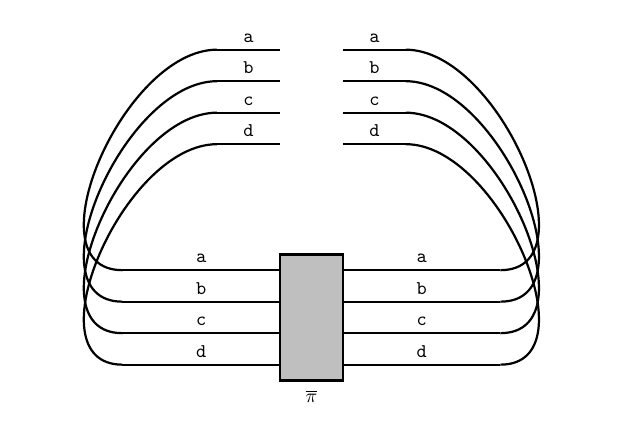
\begin{tikzpicture}[thick, scale=0.4, every node/.style={scale=0.7}]

		% Draw the wires entering the box
		\draw[-] (0, 2) -- (2, 2) node[midway, above] {\texttt{a}};
		\draw[-] (0, 1) -- (2, 1) node[midway, above] {\texttt{b}};
		\draw[-] (0, 0) -- (2, 0) node[midway, above] {\texttt{c}};
		\draw[-] (0,-1) -- (2,-1) node[midway, above] {\texttt{d}};

		% Draw the wires exiting the box with crossed mappings
		\draw[-] (4, 2) -- (6,2) node[midway, above] {\texttt{a}};
		\draw[-] (4, 1) -- (6, 1) node[midway, above] {\texttt{b}};
		\draw[-] (4, 0) -- (6, 0) node[midway, above] {\texttt{c}};
		\draw[-] (4,-1) -- (6, -1) node[midway, above] {\texttt{d}};

		\draw[-] (0-3, 2-7) to[out=180, in=180] (0, 2) node[midway, above] {};
		\draw[-] (0-3, 1-7) to[out=180, in=180] (0, 1) node[midway, above] {};
		\draw[-] (0-3, 0-7) to[out=180, in=180] (0, 0) node[midway, above] {};
		\draw[-] (0-3, -1-7) to[out=180, in=180] (0, -1)
		node[midway, above] {};

		\draw[-] (6+3, 2-7) to[out=360, in=360] (6, 2) node[midway, above] {};
		\draw[-] (6+3, 1-7) to[out=360, in=360] (6, 1) node[midway, above] {};
		\draw[-] (6+3, 0-7) to[out=360, in=360] (6, 0) node[midway, above] {};
		\draw[-] (6+3, -1-7) to[out=360, in=360] (6, -1)
		node[midway, above] {};

		% Draw the wires entering the box
		\draw[-] (0-3, 2-7) -- (2, 2-7) node[midway, above] {\texttt{a}};
		\draw[-] (0-3, 1-7) -- (2, 1-7) node[midway, above] {\texttt{b}};
		\draw[-] (0-3, 0-7) -- (2, 0-7) node[midway, above] {\texttt{c}};
		\draw[-] (0-3,-1-7) -- (2,-1-7) node[midway, above] {\texttt{d}};

		% Draw the wires exiting the box
		\draw[-] (2+2, 2-7) -- (4+5, 2-7) node[midway, above] {\texttt{a}};
		\draw[-] (2+2, 1-7) -- (4+5, 1-7) node[midway, above] {\texttt{b}};
		\draw[-] (2+2, 0-7) -- (4+5, 0-7) node[midway, above] {\texttt{c}};
		\draw[-] (2+2,-1-7) -- (4+5,-1-7) node[midway, above] {\texttt{d}};

		% Draw the lines inside the box to represent the mapping
		\draw[fill=lightgray] (2,-1.5-7) rectangle (4,2.5-7) node[midway] {};

		\node at (3, -2-7) {$\overline\pi$};


	\end{tikzpicture}
\end{center}
\noindent Turing then considered the effect of adding an edge to our menu which would have the effect of forming a loop, he called such an edge a {\bf{chain-closing constatation}}. He wanted to deduce the likelihood that adding such an edge turns our normal stops into anything other than a normal stop. We will denote this chain-closing edge as $s$. Our diagram would then be
\begin{center}
	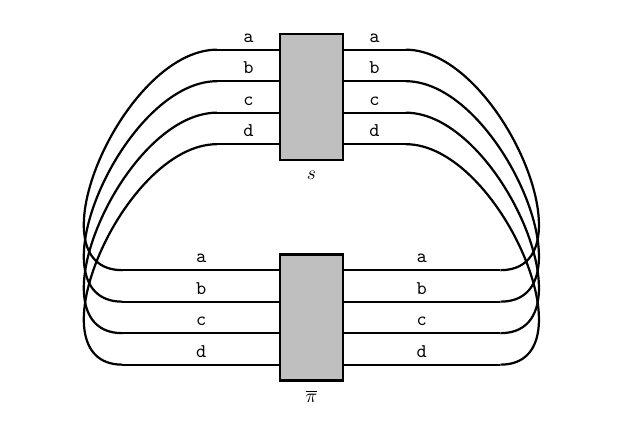
\begin{tikzpicture}[thick, scale=0.4, every node/.style={scale=0.7}]

		% Draw the lines inside the box to represent the mapping
		\draw[fill=lightgray] (2,-1.5) rectangle (4,2.5) node[midway] {};

		\node at (3, -2) {$s$};

		% Draw the wires entering the box
		\draw[-] (0, 2) -- (2, 2) node[midway, above] {\texttt{a}};
		\draw[-] (0, 1) -- (2, 1) node[midway, above] {\texttt{b}};
		\draw[-] (0, 0) -- (2, 0) node[midway, above] {\texttt{c}};
		\draw[-] (0,-1) -- (2,-1) node[midway, above] {\texttt{d}};

		% Draw the wires exiting the box with crossed mappings
		\draw[-] (4, 2) -- (6,2) node[midway, above] {\texttt{a}};
		\draw[-] (4, 1) -- (6, 1) node[midway, above] {\texttt{b}};
		\draw[-] (4, 0) -- (6, 0) node[midway, above] {\texttt{c}};
		\draw[-] (4,-1) -- (6, -1) node[midway, above] {\texttt{d}};

		\draw[-] (0-3, 2-7) to[out=180, in=180] (0, 2) node[midway, above] {};
		\draw[-] (0-3, 1-7) to[out=180, in=180] (0, 1) node[midway, above] {};
		\draw[-] (0-3, 0-7) to[out=180, in=180] (0, 0) node[midway, above] {};
		\draw[-] (0-3, -1-7) to[out=180, in=180] (0, -1)
		node[midway, above] {};

		\draw[-] (6+3, 2-7) to[out=360, in=360] (6, 2) node[midway, above] {};
		\draw[-] (6+3, 1-7) to[out=360, in=360] (6, 1) node[midway, above] {};
		\draw[-] (6+3, 0-7) to[out=360, in=360] (6, 0) node[midway, above] {};
		\draw[-] (6+3, -1-7) to[out=360, in=360] (6, -1)
		node[midway, above] {};

		% Draw the wires entering the box
		\draw[-] (0-3, 2-7) -- (2, 2-7) node[midway, above] {\texttt{a}};
		\draw[-] (0-3, 1-7) -- (2, 1-7) node[midway, above] {\texttt{b}};
		\draw[-] (0-3, 0-7) -- (2, 0-7) node[midway, above] {\texttt{c}};
		\draw[-] (0-3,-1-7) -- (2,-1-7) node[midway, above] {\texttt{d}};

		% Draw the wires exiting the box
		\draw[-] (2+2, 2-7) -- (4+5, 2-7) node[midway, above] {\texttt{a}};
		\draw[-] (2+2, 1-7) -- (4+5, 1-7) node[midway, above] {\texttt{b}};
		\draw[-] (2+2, 0-7) -- (4+5, 0-7) node[midway, above] {\texttt{c}};
		\draw[-] (2+2,-1-7) -- (4+5,-1-7) node[midway, above] {\texttt{d}};

		% Draw the lines inside the box to represent the mapping
		\draw[fill=lightgray] (2,-1.5-7) rectangle (4,2.5-7) node[midway] {};

		\node at (3, -2-7) {$\overline\pi$};


	\end{tikzpicture}
\end{center}
\noindent Suppose for a particular steckering hypothesis $S(x) = y$, the electrification of our hypothesis wire produces a normal stop. What is the probability that by adding the permutation $s$ we are now no longer in the situation of a normal stop?
\\\\Given that by supposition electrifying wire $xy$ through $\overline\pi$ has only a single live wire, the permutation $s$ need only connect the live wire to any of the $3$ remaining non-electrified wires to arrive at anything other than a normal stop. Thus there is $\frac{3}{4}$ chance that $s\circ\overline\pi$ is no longer a normal stop. Conversely, there is a $\frac{1}{4}$ chance that $s$ fails to remove our normal stop.
\\\\In the case of a $26$ character alphabet the same logic follows and we have a $\frac{1}{26}$ chance that a chain-closing constatations fails to remove a normal stop. Given that we originally expected $26^4$ normal stops over all steckering hypotheses without any closures, we would now expect that adding a chain-closing constatation to our menu would have $\frac{1}{26}$ as many normal stops. Thus adding one closure to our menu now brings the expected number of normal stops over all steckering hypotheses down to $26^{4-1} = 26^3$.
\\\\Turing extends this argument to explain that for a menu with $c$ loops (which he called {\bf{closures}}) we would expect $26^{4-c}$ normal stops over all steckering hypotheses.
\subsection{Dixon's Theorem}
A natural question arises - why should the number of normal stops over all steckering hypotheses approximate the number of stops? First, we are only considering a subset of possible stops so we might expect our approximation to be poor. Second, we are considering these stops over all steckering hypotheses so we might expect our approximation to be around $26$ times greater than the actual answer. Yet, testing Turing's formula against the actual Bombe, in many cases we find that his approximation of $26^{4-c}$ falls roughly in line with the actual number of stops. To answer this question we must show the following
\begin{enumerate}[(I)]
	\item The number of normal stops approximates the number of stops
	\item The consideration of all $26$ steckering hypotheses for each rotor position averages out in such a way that we get only $1$ steckering hypothesis per each rotor position thus removing any double counting of a particular rotor position.
\end{enumerate}
\subsubsection{Transitive Subgroups}
\noindent To show these two points, we require additional mathematical tools. We first need to translate our mechanical understanding of the Bombe's electrifcation of wires into a mathematical one. For a single loop this is quite trivial. If the permutation representing our loop is $\overline\pi$, then the number of normal stops over all steckering hypotheses is just the number of singleton cycles in $\overline\pi$'s cycle decomposition.
\\\\Once we add in additional closures this becomes slightly more complicated. Suppose we have two closures, with each seperate closure being represented by the permutations $\overline\pi$ and $\overline\delta$ respectively.
\begin{figure}[H]
	\begin{center}
		\scalebox{0.8}{
			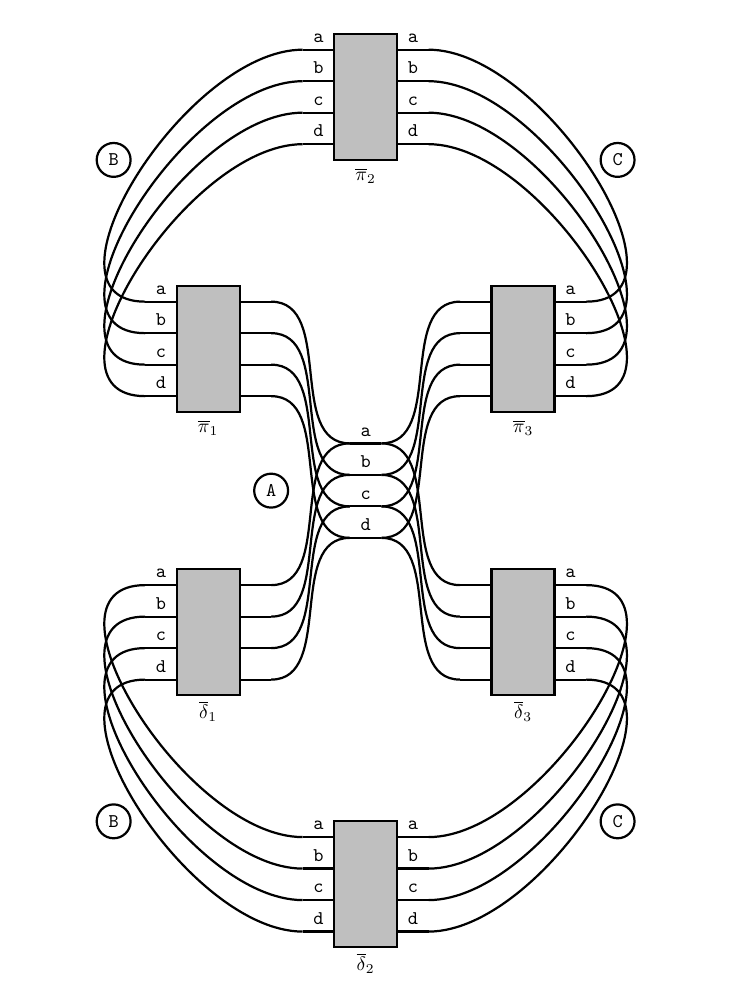
\begin{tikzpicture}[thick, scale=0.4, every node/.style={scale=0.7}]
				% Draw the box
				\draw[fill=lightgray] (0+5, 0+2) rectangle (2+5,4+2) node[midway] {};
				\node at (0+5+1, 0+2-0.5) {$\overline\pi_3$};

				% Draw the wires exiting the box
				\draw[-] (7, 5.5) -- (8,5.5) node[midway, above] {\texttt{a}};
				\draw[-] (7, 4.5) -- (8,4.5) node[midway, above] {\texttt{b}};
				\draw[-] (7, 3.5) -- (8, 3.5) node[midway, above] {\texttt{c}};
				\draw[-] (7,2.5) -- (8, 2.5) node[midway, above] {\texttt{d}};

				% Draw the wires entering the box
				\draw[-] (4, 5.5) -- (5,5.5) node[midway, above] {};
				\draw[-] (4, 4.5) -- (5,4.5) node[midway, above] {};
				\draw[-] (4, 3.5) -- (5, 3.5) node[midway, above] {};
				\draw[-] (4,2.5) -- (5, 2.5) node[midway, above] {};

				\draw[fill=lightgray] (0-5,0+2) rectangle (2-5,4+2) node[midway] {};
				\node at (0-5+1, 0+2-0.5) {$\overline\pi_1$};

				% Draw the wires entering the box
				\draw[-] (-13+7, 5.5) -- (-13+8,5.5) node[midway, above] {\texttt{a}};
				\draw[-] (-13+7, 4.5) -- (-13+8,4.5) node[midway, above] {\texttt{b}};
				\draw[-] (-13+7, 3.5) -- (-13+8, 3.5) node[midway, above] {\texttt{c}};
				\draw[-] (-13+7,2.5) -- (-13+8, 2.5) node[midway, above] {\texttt{d}};

				% Draw the wires exiting the box
				\draw[-] (-13+7+3, 5.5) -- (-13+8+3,5.5) node[midway, above] {};
				\draw[-] (-13+7+3, 4.5) -- (-13+8+3,4.5) node[midway, above] {};
				\draw[-] (-13+7+3, 3.5) -- (-13+8+3, 3.5) node[midway, above] {};
				\draw[-] (-13+7+3,2.5) -- (-13+8+3, 2.5) node[midway, above] {};

				\draw[fill=lightgray] (0,0+10) rectangle (2,4+10) node[midway] {};
				\node at (0+1, 0+10-0.5) {$\overline\pi_2$};

				% Draw the wires entering the box
				\draw[-] (-1, 3+10.5) -- (0, 3+10.5) node[midway, above] {\texttt{a}};
				\draw[-] (-1, 2+10.5) -- (0, 2+10.5) node[midway, above] {\texttt{b}};
				\draw[-] (-1, 1+10.5) -- (0, 1+10.5) node[midway, above] {\texttt{c}};
				\draw[-] (-1,0+10.5) -- (0,0+10.5) node[midway, above] {\texttt{d}};

				% Draw the wires exiting the box
				\draw[-] (3+-1, 3+10.5) -- (3+0, 3+10.5) node[midway, above]
				{\texttt{a}};
				\draw[-] (3+-1, 2+10.5) -- (3+0, 2+10.5) node[midway, above]
				{\texttt{b}};
				\draw[-] (3+-1, 1+10.5) -- (3+0, 1+10.5) node[midway, above]
				{\texttt{c}};
				\draw[-] (3+-1,0+10.5) -- (3+0,0+10.5) node[midway, above] {\texttt{d}};

				% Draw wires from 2 to 1
				\draw[-] (-6, 5.5) to[out=180, in=180] (-1, 13.5)
				node[midway, above] {};
				\draw[-] (-6, 4.5) to[out=180, in=180] (-1, 12.5)
				node[midway, above] {};
				\draw[-] (-6, 3.5) to[out=180, in=180] (-1, 11.5)
				node[midway, above] {};
				\draw[-] (-6, 2.5) to[out=180, in=180] (-1, 10.5)
				node[midway, above] {};

				% Draw wires from 3 to 2
				\draw[-] (8, 5.5) to[out=360, in=360] (3, 13.5) node[midway, above] {};
				\draw[-] (8, 4.5) to[out=360, in=360] (3, 12.5) node[midway, above] {};
				\draw[-] (8, 3.5) to[out=360, in=360] (3, 11.5) node[midway, above] {};
				\draw[-] (8, 2.5) to[out=360, in=360] (3, 10.5)
				node[midway, above] {};

				% Midway wires
				\draw[-] (0.5, 1) -- (1.5, 1) node[midway, above] {\texttt{a}};
				\draw[-] (0.5, 0) -- (1.5, 0) node[midway, above] {\texttt{b}};
				\draw[-] (0.5, -1) -- (1.5, -1) node[midway, above] {\texttt{c}};
				\draw[-] (0.5,-2) -- (1.5,-2) node[midway, above] {\texttt{d}};

				% Draw wires from 1 to midway
				\draw[-] (-2, 5.5) to[out=360, in=180] (0.5, 1) node[midway, above] {};
				\draw[-] (-2, 4.5) to[out=360, in=180] (0.5, 0) node[midway, above] {};
				\draw[-] (-2, 3.5) to[out=360, in=180] (0.5, -1) node[midway, above] {};
				\draw[-] (-2, 2.5) to[out=360, in=180] (0.5, -2) node[midway, above] {};

				% Draw wires from 2 to midway
				\draw[-] (4, 5.5) to[out=180, in=360] (1.5, 1) node[midway, above] {};
				\draw[-] (4, 4.5) to[out=180, in=360] (1.5, 0) node[midway, above] {};
				\draw[-] (4, 3.5) to[out=180, in=360] (1.5, -1) node[midway, above] {};
				\draw[-] (4, 2.5) to[out=180, in=360] (1.5, -2) node[midway, above] {};

				\draw[fill=lightgray] (0,0-15) rectangle (2,4-15) node[midway] {};
				\node at (0+1, 0+10-0.5-25) {$\overline\delta_2$};

				% Draw the wires entering the box
				\draw[-] (-1, 3+10.5-25) -- (0, 3+10.5-25) node[midway,
					above] {\texttt{a}};
				\draw[-] (-1, 2+10.5-25) -- (0, 2+10.5-25) node[midway,
					above] {\texttt{b}};
				\draw[-] (-1, 1+10.5-25) -- (0, 1+10.5-25) node[midway,
					above] {\texttt{c}};
				\draw[-] (-1,0+10.5-25) -- (0,0+10.5-25) node[midway, above]
				{\texttt{d}};

				% Draw the wires exiting the box
				\draw[-] (3+-1, 3+10.5-25) -- (3+0, 3+10.5-25) node[midway,
					above] {\texttt{a}};
				\draw[-] (3+-1, 2+10.5-25) -- (3+0, 2+10.5-25) node[midway,
					above] {\texttt{b}};
				\draw[-] (3+-1, 1+10.5-25) -- (3+0, 1+10.5-25) node[midway,
					above] {\texttt{c}};
				\draw[-] (3+-1,0+10.5-25) -- (3+0,0+10.5-25) node[midway,
					above] {\texttt{d}};

				\draw[fill=lightgray] (0-5,0+2-9) rectangle (2-5,4+2-9) node[midway] {};
				\node at (0-5+1, 0+2-0.5-9) {$\overline\delta_1$};

				% Draw the wires entering the box
				\draw[-] (-13+7, 5.5-9) -- (-13+8,5.5-9) node[midway, above]
				{\texttt{a}};
				\draw[-] (-13+7, 4.5-9) -- (-13+8,4.5-9) node[midway, above]
				{\texttt{b}};
				\draw[-] (-13+7, 3.5-9) -- (-13+8, 3.5-9) node[midway, above]
				{\texttt{c}};
				\draw[-] (-13+7,2.5-9) -- (-13+8, 2.5-9) node[midway, above]
				{\texttt{d}};

				% Draw the wires exiting the box
				\draw[-] (-13+7+3, 5.5-9) -- (-13+8+3,5.5-9) node[midway, above] {};
				\draw[-] (-13+7+3, 4.5-9) -- (-13+8+3,4.5-9) node[midway, above] {};
				\draw[-] (-13+7+3, 3.5-9) -- (-13+8+3, 3.5-9) node[midway, above] {};
				\draw[-] (-13+7+3,2.5-9) -- (-13+8+3, 2.5-9) node[midway, above] {};

				% Draw the box
				\draw[fill=lightgray] (0+5, 0+2-9) rectangle (2+5,4+2-9)
				node[midway] {};
				\node at (0+5+1, 0+2-0.5-9) {$\overline\delta_3$};

				% Draw the wires exiting the box
				\draw[-] (7, 5.5-9) -- (8,5.5-9) node[midway, above] {\texttt{a}};
				\draw[-] (7, 4.5-9) -- (8,4.5-9) node[midway, above] {\texttt{b}};
				\draw[-] (7, 3.5-9) -- (8, 3.5-9) node[midway, above] {\texttt{c}};
				\draw[-] (7,2.5-9) -- (8, 2.5-9) node[midway, above] {\texttt{d}};

				% Draw the wires entering the box
				\draw[-] (4, 5.5-9) -- (5,5.5-9) node[midway, above] {};
				\draw[-] (4, 4.5-9) -- (5,4.5-9) node[midway, above] {};
				\draw[-] (4, 3.5-9) -- (5, 3.5-9) node[midway, above] {};
				\draw[-] (4,2.5-9) -- (5, 2.5-9) node[midway, above] {};

				% Draw wires from 4 to 5
				\draw[-] (-6, 5.5-9) to[out=180, in=180] (-1, 13.5-25)
				node[midway, above] {};
				\draw[-] (-6, 4.5-9) to[out=180, in=180] (-1, 12.5-25)
				node[midway, above] {};
				\draw[-] (-6, 3.5-9) to[out=180, in=180] (-1, 11.5-25)
				node[midway, above] {};
				\draw[-] (-6, 2.5-9) to[out=180, in=180] (-1, 10.5-25)
				node[midway, above] {};

				% Draw wires from 5 to 6
				\draw[-] (8, 5.5-9) to[out=360, in=360] (3, 13.5-25)
				node[midway, above] {};
				\draw[-] (8, 4.5-9) to[out=360, in=360] (3, 12.5-25)
				node[midway, above] {};
				\draw[-] (8, 3.5-9) to[out=360, in=360] (3, 11.5-25)
				node[midway, above] {};
				\draw[-] (8, 2.5-9) to[out=360, in=360] (3, 10.5-25)
				node[midway, above] {};

				% Draw wires from 4 to midway
				\draw[-] (-2, 5.5-9) to[out=360, in=180] (0.5, 1)
				node[midway, above] {};
				\draw[-] (-2, 4.5-9) to[out=360, in=180] (0.5, 0)
				node[midway, above] {};
				\draw[-] (-2, 3.5-9) to[out=360, in=180] (0.5, -1)
				node[midway, above] {};
				\draw[-] (-2, 2.5-9) to[out=360, in=180] (0.5, -2)
				node[midway, above] {};

				% Draw wires from 2 to midway
				\draw[-] (4, 5.5-9) to[out=180, in=360] (1.5, 1) node[midway, above] {};
				\draw[-] (4, 4.5-9) to[out=180, in=360] (1.5, 0) node[midway, above] {};
				\draw[-] (4, 3.5-9) to[out=180, in=360] (1.5, -1)
				node[midway, above] {};
				\draw[-] (4, 2.5-9) to[out=180, in=360] (1.5, -2)
				node[midway, above] {};
				\node[draw,circle] at (-2, -0.5) {\texttt{A}};
				\node[draw,circle] at (-7, -11) {\texttt{B}};
				\node[draw,circle] at (-7, -11+21) {\texttt{B}};
				\node[draw,circle] at (-7+16, -11) {\texttt{C}};
				\node[draw,circle] at (-7+16, -11+21) {\texttt{C}};

			\end{tikzpicture}
		}
	\end{center}
\end{figure}
\noindent How can we determine which wires are connected to which in this complex arrangment of permutations? To answer this we introduce
\begin{definition}
	The subgroup of $S_n$ generated by two permutations $\sigma$, $\tau$ $\in S_n$ is
	\begin{center}
		$\langle\sigma,\tau\rangle \coloneq \{\sigma^{a_1}\tau^{b_1}\dots\sigma^{a_k}\tau^{b_k}\text{ }|\text{ }k\in\mathbb{N},\text{ }a_i,b_i\in\mathbb{Z}\}$
	\end{center}
\end{definition}
\noindent This is the set of all group elements obtained by applying finite compositions of $\sigma$, $\tau$, and their inverses.
\\\\Consider how this relates to our two loop Bombe arrangment with $\overline\pi$ and $\overline\delta$. The electricity is free to flow through any number of iterations forwards and backwards through both $\overline\pi$ and $\overline\delta$. Applying a current at some input wire will propogate in such a way that it reaches possible letters which can be reached by some sequence of applications of $\overline\pi$, $\overline\delta$, and their inverses. Then on cable \texttt{A}, applying a current at some input $x$ can only reach wire $y$ on that cable if $\exists\text{ }\sigma\in\langle\overline\pi, \overline\delta\rangle$ such that $\sigma(x) = y$. If we want to know for a given input wire, what other wires it can reach, we need to know which letters are connected to which through permutations in $\langle\overline\pi, \overline\delta\rangle$.
\\\\We note that $\langle\overline\pi, \overline\delta\rangle$ has a natural group action on $\mathbb{N}_{4}$ given by
\begin{align*}
	\sigma\cdot{x} \coloneq \sigma(x)\text{ for }\sigma\in\langle\overline\pi, \overline\delta\rangle\text{ and }x\in\mathbb{N}_{4}.
\end{align*}
Consider an orbit for this group action. That is, for $x\in\mathbb{N}_{4}$ we have
\begin{center}
	$\langle\overline\pi, \overline\delta\rangle\cdot x\coloneq\{\sigma(x)\text{ }|\text{ }\sigma\in\langle\overline\pi, \overline\delta\rangle\}$
\end{center}
\noindent We can think of this orbit as all elements in $\mathbb{N}_{4}$ which $x$ can reach via some sequence finite compositions of $\overline\pi$, $\overline\delta$, and their inverses. This is exactly analogous to the set of wires on cable \texttt{A} which can be reached from an input on $x$. Then these orbits partition $\mathbb{N}_{4}$ and tell us which wires are in a connected loop in our Bombe arrangement.
\\\\In this way the parition given by the set of orbits $\mathbb{N}_{4}/\langle\overline\pi, \overline\delta\rangle$ represents which wires are connected to which wires in our diagram. If $\mathbb{N}_{4}/\langle\overline\pi, \overline\delta\rangle = \{\{\texttt{a},\dots,\texttt{d}\}\}$ then we know that electrifying any wire on cable \texttt{A} will electrify all wires in the diagram. In such a case we say that $\langle\overline\pi, \overline\delta\rangle$ forms a {\bf{transitive subgroup}} of $S_4$. Formally,
\begin{definition}
	Let $H\le{G}$ be a sub-group of $G$ which acts on a set $X$. We say $H$ acts {\bf{transitively}} on $S\subseteq{X}$ provided that
	\begin{center}
		$\forall\text{ }a,b\in S\text{, }\exists\text{ }\sigma\in{H}\text{ s.t. }\sigma(a)=b$.
	\end{center}
	If $H$ acts transitively on $X$ we say that $H$ is a {\bf{transitive subgroup of $G$}}.
\end{definition}
\noindent Consider how this relates to our single loop example.
\begin{center}
	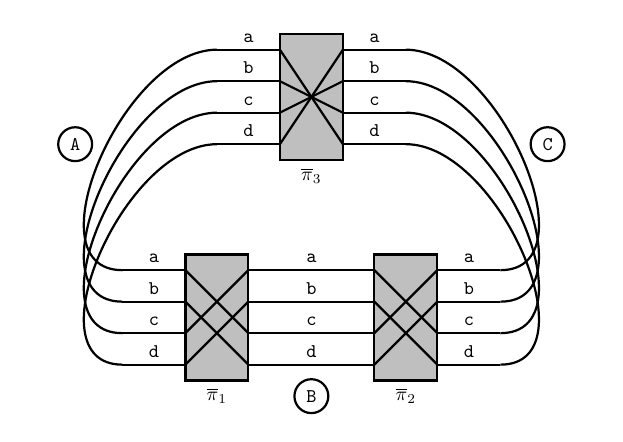
\begin{tikzpicture}[thick, scale=0.4, every node/.style={scale=0.7}]
		% Draw the box
		\draw[fill=lightgray] (2,-1.5) rectangle (4,2.5) node[midway] {};

		\node at (3, -2) {$\overline\pi_3$};

		% Draw the wires entering the box
		\draw[-] (0, 2) -- (2, 2) node[midway, above] {\texttt{a}};
		\draw[-] (0, 1) -- (2, 1) node[midway, above] {\texttt{b}};
		\draw[-] (0, 0) -- (2, 0) node[midway, above] {\texttt{c}};
		\draw[-] (0,-1) -- (2,-1) node[midway, above] {\texttt{d}};

		% Draw the wires exiting the box with crossed mappings
		\draw[-] (4, 2) -- (6,2) node[midway, above] {\texttt{a}};
		\draw[-] (4, 1) -- (6, 1) node[midway, above] {\texttt{b}};
		\draw[-] (4, 0) -- (6, 0) node[midway, above] {\texttt{c}};
		\draw[-] (4,-1) -- (6, -1) node[midway, above] {\texttt{d}};

		% Draw the lines inside the box to represent the mapping
		\draw[-] (2, 2) -- (4,-1);
		\draw[-] (2, 1) -- (4, 0);
		\draw[-] (2, 0) -- (4, 1);
		\draw[-] (2,-1) -- (4, 2);

		\draw[-] (0-3, 2-7) to[out=180, in=180] (0, 2) node[midway, above] {};
		\draw[-] (0-3, 1-7) to[out=180, in=180] (0, 1) node[midway, above] {};
		\draw[-] (0-3, 0-7) to[out=180, in=180] (0, 0) node[midway, above] {};
		\draw[-] (0-3, -1-7) to[out=180, in=180] (0, -1)
		node[midway, above] {};

		\draw[-] (6+3, 2-7) to[out=360, in=360] (6, 2) node[midway, above] {};
		\draw[-] (6+3, 1-7) to[out=360, in=360] (6, 1) node[midway, above] {};
		\draw[-] (6+3, 0-7) to[out=360, in=360] (6, 0) node[midway, above] {};
		\draw[-] (6+3, -1-7) to[out=360, in=360] (6, -1)
		node[midway, above] {};

		\draw[fill=lightgray] (2-3,-1.5-7) rectangle (4-3,2.5-7) node[midway] {};

		\node at (3-3, -2-7) {$\overline\pi_1$};

		% Draw the wires entering the box
		\draw[-] (0-3, 2-7) -- (2-3, 2-7) node[midway, above] {\texttt{a}};
		\draw[-] (0-3, 1-7) -- (2-3, 1-7) node[midway, above] {\texttt{b}};
		\draw[-] (0-3, 0-7) -- (2-3, 0-7) node[midway, above] {\texttt{c}};
		\draw[-] (0-3,-1-7) -- (2-3,-1-7) node[midway, above] {\texttt{d}};

		% Draw the wires exiting the box
		\draw[-] (4-3, 2-7) -- (6-3,2-7) node[right, above] {\texttt{a}};
		\draw[-] (4-3, 1-7) -- (6-3, 1-7) node[right, above] {\texttt{b}};
		\draw[-] (4-3, 0-7) -- (6-3, 0-7) node[right, above] {\texttt{c}};
		\draw[-] (4-3,-1-7) -- (6-3, -1-7) node[right, above] {\texttt{d}};

		% Draw the lines inside the box to represent the mapping
		\draw[-] (2-3, 2-7) -- (4-3, 0-7);
		\draw[-] (2-3, 1-7) -- (4-3, -1-7);
		\draw[-] (2-3, 0-7) -- (4-3, 2-7);
		\draw[-] (2-3,-1-7) -- (4-3, 1-7);

		\draw[fill=lightgray] (2+3,-1.5-7) rectangle (4+3,2.5-7) node[midway] {};

		\node at (3+3, -2-7) {$\overline\pi_2$};

		% Draw the wires entering the box
		\draw[-] (0+3, 2-7) -- (2+3, 2-7) node[midway, above] {};
		\draw[-] (0+3, 1-7) -- (2+3, 1-7) node[midway, above] {};
		\draw[-] (0+3, 0-7) -- (2+3, 0-7) node[midway, above] {};
		\draw[-] (0+3,-1-7) -- (2+3,-1-7) node[midway, above] {};

		% Draw the wires exiting the box
		\draw[-] (4+3, 2-7) -- (6+3,2-7) node[midway, above] {\texttt{a}};
		\draw[-] (4+3, 1-7) -- (6+3, 1-7) node[midway, above] {\texttt{b}};
		\draw[-] (4+3, 0-7) -- (6+3, 0-7) node[midway, above] {\texttt{c}};
		\draw[-] (4+3,-1-7) -- (6+3, -1-7) node[midway, above] {\texttt{d}};

		\draw[-] (2+3, 2-7) -- (4+3, 0-7);
		\draw[-] (2+3, 1-7) -- (4+3, -1-7);
		\draw[-] (2+3, 0-7) -- (4+3, 2-7);
		\draw[-] (2+3,-1-7) -- (4+3, 1-7);
		\node[draw,circle] at (-4.5, -1) {\texttt{A}};
		\node[draw,circle] at (3, -9) {\texttt{B}};
		\node[draw,circle] at (10.5, -1) {\texttt{C}};
	\end{tikzpicture}
\end{center}
\noindent In this loop, we have that on cable \texttt{A}, wires \texttt{a} and \texttt{d} are connected, and wires \texttt{b} and \texttt{c} are connected. We explained that his could be simply determined by examining the cycle decomposition of $\overline\pi$ which in this case is
\begin{center}
	(\texttt{ad})(\texttt{bc})
\end{center}
\noindent However, we can get the exact same picture by simply considering the set orbits of $\langle\overline\pi\rangle$ acting on $\{\texttt{a},\dots\texttt{z}\}$, which would give us
\begin{center}
	$\{\{\texttt{a}, \texttt{d}\},\{\texttt{b}, \texttt{c}\}\}$
\end{center}
\noindent which gives us an equal picture of the connections between wires on the \texttt{A} cable. Additionally, shifting to this view means that rather than saying the entire loop becomes electrified when $\overline\pi$ has a $26^1$ cycle type, we say that this occurs when $\langle\overline\pi\rangle$ forms a transitive subgroup of $S_4$.
\\\\This description is more robust in that it can handle any number of closures and gives us a picture of which wires are connected to which on a particular cable.
\subsubsection{Distribution of Stops}
Equipped with this mathematical framework are now ready to address Turing's model. We will classify stops by the cardinality and multiplicty of sets in the partition given by the orbits described above. For example, if a set of orbits is
\begin{center}
	$\{\{\texttt{a}, \dots, \texttt{m}\}, \{\texttt{n}, \dots, \texttt{z}\}\}$
\end{center}
we would say this stop is a $13^2$ stop. This is effectively analogous to the cycle type of a permutation but in order to extend this to multiple loops we must frame it in this description of partitions given by orbits of subgroups. We will call these orbit structures.
\\\\In Turing's model, such a $13^2$ stop as above, would count as $0$ normal stops over all steckering hypotheses. In the actual running of the Bombe this would constitute a single stop. Further, a $1^323^1$ stop in Turing's model would be considered as $3$ normal stops over all possible steckering hypotheses. In reality this would only constitute a single real stop in the running of the Bombe. This highlights the two qualms that we are trying to reconcile in Turing's model, the absence of abnormal stops, and the overcounting of normal stops.
\\\\We begin by considering the case of $2$ closures, where at each rotor position of the Bombe, we have some permutations $\overline\pi$ and $\overline\delta$. What is the distribution of stop types? For now we will assume that any loop in a particular configuration of the Bombe represents a random permutation. We will later refine this, but as a heuristic it serves to justify Turing's model. We want to know what stop types are most common. That is, given two random permutations $\overline\pi$ and $\overline\delta$, what is the distribution of orbit structures for the subgroup $\langle\overline\pi, \overline\delta\rangle$? This question was answered by John Dixon in 1969 in his paper ``The Probability of Generating the Symmetric Group''.

\begin{theorem}[Dixon's Theorem]
	Given two random permutations $\sigma$ and $\tau$ in $S_n$, the probability that $\langle\sigma, \tau\rangle$ have an orbit structure of $1^{m_1}\dots n^{m_n}$ is
	\begin{align*}
		1-\frac{1}{n!}\sum_{1^{\ell_1}\dots n^{\ell_n} \ne 1^{m_1}\dots n^{m_n}}\prod_{i=1}^n{\frac{(i!t_{i})^{\ell_i}}{\ell_i!}}
	\end{align*}
	where $t_i$ is the probability that two random permutations in $S_i$ form a transitive subgroup.
\end{theorem}
\begin{proof}
	Let $t_i$ be the probability that for two random $x,y\in S_i$, we have that $\langle x,y\rangle$ acts transitively on $\mathbb{N}_i$.
	\\\\Fix a partition $\omega_1\cup\dots\cup\omega_k$ of $\mathbb{N}_n$. We want to know the number of $x,y\in S_n$ such that $\langle x,y\rangle$ have orbits which are exactly the sets in our partition. For $\langle x, y\rangle$ to contain an orbit $\omega_i$, we must have that $\langle x,y\rangle$ acts transitively on $\omega_i$. That is, $\forall$ $a,b\in\omega_i$\text{ }$\exists\text{ }\sigma\in\langle x,y\rangle$ such that $\sigma(a) = b$. This also means that the restriction of the action $\langle x,y\rangle$ to $\omega_i$ is a transitive group action.  The total number of restrictions to $\omega_i$ without any constraints on transitivity is $(|\omega_i|!)^2$, so to get the number of restrictions which represent a transitive action we compute $(|\omega_i|!)^2t_{|\omega_i|}$. To contain all orbits $\omega_i$, we must have that when restricted to each $\omega_i$, $\langle x,y\rangle$ acts transitively. Thus there are
	\begin{center}
		$\prod_{i=1}^k(|\omega_i|!)^2t_{|\omega_i|}$
	\end{center}
	permutations $x,y\in S_n$ such that $\langle x,y\rangle$ has an orbit structure equivalent to the partition $\omega_1\cup\dots\cup\omega_k$.
	\\\\Supposing we have a particular partition with $ell_i$ sets of size $i$ then our above argument can be framed as stating that there are
	\begin{center}
		$\prod_{i=1}^n{((i!)^2t_i)^{\ell_i}}$
	\end{center}
	The number of partitions with $\ell_i$ sets of size $i$ is exactly
	\begin{center}
		$\frac{n!}{\prod_{i=1}^n{(i!)^{\ell_i}\ell_i!}}$
	\end{center}
	We compute the probability that $x,y\in S_n$ do \emph{not} generate an orbit structure with $m_i$ orbits of size $i$, by computing the total number of $x,y\in S_n$ which generate any other orbit structure, and dividing by $(n!)^2$ (i.e. the total number of pairs of permutations in $S_n$). This is precisely
	\begin{align*}
		          & \sum_{1^{\ell_1}\dots n^{\ell_n} \ne 1^{m_1}\dots n^{m_n}}{\frac{1}{(n!)^2}\frac{n!}{\prod_{i=1}^n{(i!)^{\ell_i}\ell_i!}}}\prod_{i=1}^n{((i!)^2t_i)^{\ell_i}} \\
		=\text{ } & \frac{1}{n!}\sum_{1^{\ell_1}\dots n^{\ell_n} \ne 1^{m_1}\dots n^{m_n}}{\prod_{i=1}^n{\frac{(i!)^{2\ell_i}t_i^{\ell_i}}{(i!)^{\ell_i}\ell_i!}}}                \\
		=\text{ } & \frac{1}{n!}\sum_{1^{\ell_1}\dots n^{\ell_n} \ne 1^{m_1}\dots n^{m_n}}{\prod_{i=1}^n{\frac{(i!)^{\ell_i}t_i^{\ell_i}}{
		\ell_i!}}}
	\end{align*}
	The opposite of this probability is the probability that we generate exactly the orbit structure we specified, thus giving us the desired result.
\end{proof}
\noindent It should be noted that the actual statement of this proof is a formula for $t_n$ which is then shown to asymptotically approach $1$ as $n$ increases. In the context of the theorem above, $t_n$ can be solved by computing the probability that $\langle \sigma, \tau\rangle$ have an orbit structure of $26^1$, that is, the subgroup formed is transitive. For such an orbit structure, each $t_i$ given in our equation necessarily has $i < n$ so we can recursively solve for $t_n$. With the ability to solve for any $t_k$ for $k\in\mathbb{N}$ we can then go and compute the probability of any particular orbit structure via the above theorem.
\subsection{Turing's Model's Accuracy}\label{justify_turing}
We can now compute for the case of two loops, what the probability of a particular stop type is. Computing the above for a $26^1$ orbit structure tells us that roughly $95.9\%$ of all rotor configurations in a two loop structure will electrify all wires, producing no stop whatsoever. The remaining $4.1\%$ of rotor configurations account for all possible stops. Of these stops we can compute that roughly $92.3\%$ of these stops have a stop type of $1^125^1$. This is a \emph{massive} proportion of the possible stops. Nearly all stops have this singular stop type, and herein lies the justification for Turing's method.
\\\\For the sake of argument, suppose \emph{all} stops were of the type $1^125^1$. In this case, we note two observations
\begin{enumerate}[(I)]
	\item All stops have a normal stops
	\item The number of steckering hypothesis producing a normal stop for each stop type is $1$
\end{enumerate}
It would then follow that if we could compute the number of normal stops over all steckering hypothesis we would get exactly the number of total stops. In such a case Turing's calculation of the expected number of normal stops over all steckering hypothesis is the same as the expected number of stops. As the proportion of stops whose stop type is $1^125^1$ increases, Turing's expected number of normal stops over all steckering hypothesis will begin to align with the total number of actual stops. Given that $92.3\%$ of stops have this stop type with just two closures, we can expect that Turing's estimate is very strong.
\\\\As the number of closures increases, such an estimate improves. This is because for $\langle \sigma_1, \dots, \sigma_k\rangle\le S_{26}$, the expected size of orbits should increase as $k$ increases. This can be shown heuristically via the orbit-stabilizer theorem which tells us that
\begin{theorem}[Orbit-Stabilizer Theorem]
	For a group $G$ acting on a finite set $X$, we have that for $x\in X$
	\begin{align*}
		|G\cdot x| = \frac{|G|}{|G_x|}
	\end{align*}
	where $G\cdot x$ is the orbit of $x$ and $G_x$ is the stabilizer of $x$.
\end{theorem}
\noindent We see that the size of the orbit of $x$ is inversely proportional to the size of its stabilizer. As we increase the number of random permutations generating our subgroup, the  constraints required for an element to fix $x$ become increasingy unlikely to be satisified by independent random generators. Thus we expect the average size of $G_x$ to go down and thus the average size of an orbit increases. In our context, this means that with more closures, Turing's estimate approaches the true number of stops.

\subsubsection{Simulating Turing's Model}
We will now show to what extent Turing's model aligns with ground-truth simulation. For testing during this thesis I created a simulation of both the Bombe and the Enigma machine. However, to ensure my implict biases regarding my understanding of the Bombe's functions do not interfere with my analysis, to provide simulated figures of the Bombe we will use Jean-François Bouchaudy's simulation of the Bombe. This simulation in its current form misses a number of stops that were detected by my simulation since, for poorer menus, it fails to propogate the input singal sufficiently to reach a steady state. If we increase the propogation to $100$ loops per position of the Bombe then my simulation falls in line with Bouchaudy's.
\\\\We can run Bouchaudy's simulation with randomly generated menu configurations and rotor choices, allowing us to compute the average number of stops along with a margin of error with $95\%$ confidence.
\\\\ For instance, running a monte carlo simulation of menus with three closures, we find that there are $30.26\pm0.57$ stops. Turing's estiamte would give us $26^{4-3}$ or $26$ stops which, tough outside the margin of error, is still relatively close the the simulated ground-truth.
\\\\However, as we remove closures, we can expect that the distribution of stop types will diverge away from $1^125^1$ stops, and Turing's estimate will stray from the actual number of stops. This can be seen by running a menu with a single closure which produces $17003.50\pm23.83$ stops. Turing's estimate would give us $26^{4-1}$ or $17576$ stop which falls far outside the desired margin of error of simulation.
\\\\Turing's estimate is a strong heuristic model for the number of stops, but we can see that even with a large number of closures, his model is not accurate enough to fit within our desired margin of error. Were the Enigma machine to use more letters, or the number of closures to be significantly higher, we would expect Turing's model to fall within the margin of error; However, in the case of a $26$ letter alphabet, with only a few closures, the number of abnormal stops and the number of stops with multiple steckering hypotheses producing normal stops are too high for the model to align with reality. In order to address these problems, we must develop a new model which does away with some of Turing's fundamental assumptions.
\section{The Cycle-Type Model}
The goal of Turing's model was to compute the expected number of normal stops over all steckering hypotheses. In the last section, we justified that for stronger menus, this serves as a reasonable estimate for the true number of stops but still failed to capture the accuracy desired. The goal for this section is to produce a model which considers \emph{all} stops, not just normal stops.
\\\\Further, in order to justify Turing's model, we made use of Dixon's theorem which showed that for two random permutations the probability they cause a $1^125^1$ stop type is sufficiently high to explain Turing's model's convergence to our simulation. In reality, the permutations formed by the scramblers on the Bombe are not random, but rather form a complex distribution that must be factored into our model to most accurately mimic the simulated behavior.
\subsection{Single Loop} Consider a Bombe running a menu with a single closure. This closure is made up of some number of scramblers which we denote $\overline\pi_1, \dots, \overline\pi_\ell$. In the loop these form one permutation $\overline\pi = \overline\pi_1\dots\overline\pi_\ell$. The Bombe will stop whenever $\overline\pi$ fails to connect all wires in the Bombe. We have previously shown that this occurs whenever $\overline\pi$ is not a $26$, or equivalently, whenever $\langle\overline\pi\rangle$ does not form a transitive subgroup of $S_{26}$.
\\\\We might expect that composing $\ell$ scramblers should produce a reasonably a permutation $\overline\pi$ that is relatively random in $S_{26}$. If this was the case, we would expect $\overline\pi$ to be a $26$ cycle with probability $\frac{1}{26}$ and thus we would expect a stop with probability $\frac{25}{26}$. Thus over $26^3$ possible rotor positions, we would expect $26^2\cdot25 = 16900$ stops.
\\\\Running our simulation with $\ell = 5$ we find that there are $16224.77\pm2.80$ stops. This is significantly off from our prediction. Further, a simulation with $\ell=4$ produces $17576$ stops with no margin of error, meaning that \emph{every} position on \emph{every} menu with this structure produces a stop. Clearly, we are not dealing with permutations $\overline\pi$ that are random.

\subsubsection{Parity}
To make this clear, consider our case where $\ell=4$. We have $4$ permutations $\overline\pi_1,\dots, \overline\pi_4$ which make up our loop $\overline\pi$. Each permutation $\overline\pi_i$ is a permutation representing an Enigma machine meaning that it has a $2^{13}$ cycle. This means that each permutation in our loop is made of $13$ disjoint transpositions. This means that each permutation $\overline\pi_i$ has an odd parity. Thus the composition of $4$ such permutations of odd parity must result in a permutation of even parity. Given that any $26$ cycle is necessarily of odd parity. Thus $\overline\pi$ can \emph{never} be have cycle type $26^1$ and thus always produces a stop. In mathematical terms, we would say the distribution generated by composing $4$ of these Enigma permutations is support on $A_{26}$ -- the set of even permutations in $S_{26}$. In fact, this is true for any loop where $\ell$ is even.
\\\\Similarly, for any odd $\ell$, $\overline\pi$ cannot produce any even parity cycle types, including our $1^125^1$ stop type that was so common in the two cycle case. In this case, the distribution is support on odd permutations $S_{26}-A_{26}$.
\\\\The important takeaway is that we cannot just consider the number of closures in a menu -- we must also consider the length of each loop within the closures of a menu. The length of a closure completely changes which set our distribution is supported on. Thus, our model will aim to express this by factoring in the additional variable of closure length.
\subsubsection{Simulating the One-Loop Case}
The distribution generated by composing permutations (in our case $2^{13}$ cycles) is a deeply complicated subject that is out of the scope of this paper. The relationship between $\ell$ and the resulting distribution in $S_{26}$ is so complex and vast in its possible enumeration that our best chance at getting a reasonable grasp of this distribution is to simulate it.
\\\\The use of a simulation to get the expected number of stops for a single loop of length $\ell$ begs the following questions
\begin{enumerate}
	\item[(1)] If we can simulate the number of expected stops for one closure, why not just solve the entire problem of computing the expected number of stops via simulation?
\end{enumerate}
While we might be able to run a lengthy Monte Carlo simulation of the Bombe over many different menu arrangements and shapes, the nature of the Bombe is so complicated that in practice there is no convergence to a steady state. Focusing on a single loop allows us to reach a distribution with a steady state fairly quickly. We can then rely on this distribution to compute more complicated menu arrangments which we will discuss in the following section.
\\\\In practice, this distribution was reached by running a Monte Carlo simulation. In each iteration, we initialize $\ell$ Enigma machines with the \texttt{pyenigma} package. Each had the same randomized rotor ordering and window setting, then each machine was given a randomized offset, and the resulting cycle type of their composition was collected. As we collect this distribution, we compute the total variation distance change between our distributions every $1000$ iterations. If the total variation distance change between our distributions goes below $0.00001$ for more than $30$ comparisons, we deem that the distribution has reached a steady state.
\\\\Implicit in this simulation is the assumption that permutations produced by the Bombe are uniformly distributed within each cycle type. This is a reasonable assumption since all permutations for a given cycle type are the same up to relabelling. Therefore, we expect no structural differences within the distribution for a fixed type.
\\\\Initially, we initialized $\ell$ permutations chosen randomly from the set of permutations with cycle type $2^{13}$ to perform our simulation. However, when we looked at the two closure case, certain edge cases, such as the case where one closure is of length $2$, strayed from the simulated results. This is likely because the Enigma machines being represented in the Bombe all have the same initial configuration, only with different offsets, meaning that the permutations they represent are not purely independent $2^{13}$ permutations and there is some complicated underlying statistical relationship between the permutations in a loop. 
\begin{enumerate}
	\item[(2)]Would cryptanalysts at the time be able to simulate such a distribution?
\end{enumerate}
While cryptanalysts at the time may not have been able to simulate as many iterations as we can with modern computers, we do know that such technology existed as would make this task reasonably achievable at the time. Recall from section \ref{cyclometer}, that the Polish Cipher Beaurea produced a device called the cyclometer, whose sole purpose was to quickly determine the cycle type produced by composing two Enigma permutations. With simple changes this could easily be extended to determine cycle types of arbitrary length loops of Enigma machines. With some random sampling and tedious cataloguing, it is certainly feasible that cryptanalysts of the time could have computed a distribution close to the one discussed in this section.
\subsubsection{One Loop Results}
With both these points addressed, we can examine the results of simulating a single loop of length $\ell$. After collecting the cycle distribution for each length $\ell$ over a large Monte Carlo simulation, we can take the sum of observed frequency which are not $26^1$ cycles as our probability of a stop occuring. Multiplying this by $26^3$ we get our expected number of stops. We then compare this with a small simulation run via Bouchaudy's simulation as our ground truth. 
\begin{table}[H]
\centering

\begin{tabular}{|c|c|c|}
\hline
{\bf{ $l$ }} & {\bf{ Expected Stops }} & {\bf{ Simulated Stops }}\\
\hline
2 & 17576.00 & $17576.00 \pm 0.00$\\
\hline
3 & 16246.63 & $16243.78 \pm 6.91$\\
\hline
4 & 17576.00 & $17576.00 \pm 0.00$\\
\hline
5 & 16224.88 & $16220.57 \pm 6.66$\\
\hline
6 & 17576.00 & $17576.00 \pm 0.00$\\
\hline
7 & 16222.69 & $16224.37 \pm 6.63$\\
\hline
8 & 17576.00 & $17576.00 \pm 0.00$\\
\hline
9 & 16223.75 & $16227.80 \pm 6.92$\\
\hline
10 & 17576.00 & $17576.00 \pm 0.00$\\
\hline
11 & 16224.53 & $16228.59 \pm 6.95$\\
\hline
12 & 17576.00 & $17576.00 \pm 0.00$\\
\hline
\end{tabular}
\caption{Single-Loop Bombe Stop Probabilities for Loop Lengths $l=2$ to $l=12$}
\end{table}
\noindent It is no surprise that these two values line up with each others since they are both just simulated implementations of the Bombe, but we will see that with just this small simulation, we are able to accurately estimate the stops for the case of two loops, without the need for any further simulation.
\subsection{Two Loops}
Consider a Bombe running a menu with two closures. These closures are made up of two sets of scramblers we denote $\overline\pi_1, \dots, \overline\pi_r$ and $\overline\delta_1,\dots,\overline\delta_s$ -- forming two loops with permutations $\overline\pi$ and $\overline\delta$. The Bombe will stop whenever these permutations fail to connect all wires in the Bombe. We have previously shown that this occurs whenever $\langle \overline\pi, \overline\delta \rangle$ does not form a transitive subgroup of $S_{26}$.
\\\\To get the expected number of stops we need only know the probability that $\langle \overline\pi, \overline\delta \rangle$ form a transitive subgroup. If $\overline\pi$ and $\overline\delta$ were uniformly distributed in $S_{26}$ this question would be easily answered via Dixon's theorem; However, we just showed that these permutations are not evenly distributed and their distributions are dependent on the lengths $s$ and $r$. In the last section, we gathered the distribution for each length $\ell$, so we know the probability that a particular cycle type $1^{m_1}\dots26^{m_{26}}$ occurs for a loop of length $\ell$.
\\\\Therefore, we will approach this problem by finding the probability that two permutations pulled uniformly from two fixed cycle types form a transitive subgroup of $S_{26}$.
\\\\We will first simplify our notation to make such a problem easier to state formally. Rather than denoting a cycle type as $1^{m_1}\dots n^{m_{n}}$, we will instead shorten this to the sequence of multiplicities $m=(m_i)$, where $i$ ranges from $1$ to $n$, to mean that this permutation has an $m_i$ many $i$ cycles. We will then denote $t_{\alpha, \beta} =t_{(\alpha_i), (\beta_i)}$ as the probability that a random permutation with cycle type $\alpha =(\alpha_i)$, and a random permutation with cycle type $\beta = (\beta_i)$, form a transitive subgroup. This collapses our notations of cycle type into a single variable that will make notation signficantly more condensed. 
\\\\Assuming we have a means to compute these $t_{\alpha, \beta}$, we can then introduce our single loop distribution from the last section to compute
\[
	\mathbb{P}(\overline\pi\text{ has cycle type }\alpha)\cdot\mathbb{P}(\overline\delta\text{ has cycle type }\beta)\cdot t_{\alpha, \beta}
\]
This is the probability that $\overline\pi$ has a fixed cycle type $\alpha$ and $\overline\delta$ has a fixed cycle type $\beta$, and that these two permutations form a transitive subgroup. To get the probability that any two $\overline\pi$ and $\overline\delta$ form a transitive subgroup, we can simply range over all possible cycle types to get
\begin{align*}
	 & \mathbb{P}(\langle \overline\pi,\overline\delta \rangle\text{ forms a transitive subgroup})
	\\= &\sum_{\alpha, \beta}\mathbb{P}(\overline\pi\text{ has cycle type }\alpha)\cdot\mathbb{P}(\overline\delta\text{ has cycle type }\beta)\cdot t_{\alpha, \beta}
\end{align*}
and the inverse of this probability will be the probability of a stop. 
\\\\Then we need only to compute these $t_{\alpha, \beta}$ to solve the two loop case. In order to do this, we must modify Dixon's theorem to be expressed in terms of cycle types rather than the size of the ambient space.
\subsubsection{Computing $t_{\alpha, \beta}$}
In order to solve this problem, just as in Dixon's theorem, we will enumerate partitions of $\mathbb{N}_n$. \\\\Let
\[
\mathcal{P}_n \coloneqq \left\{ \{ \omega_1, \dots, \omega_k \} \,\middle|\, k \in \mathbb{N},\ \omega_i \neq \emptyset,\ \omega_i \cap \omega_j = \emptyset\ \text{for } i \neq j,\ \bigcup_{i=1}^k \omega_i = \mathbb{N}_n \right\}
\]be the set of partitions of \( \mathbb{N}_n \). 
\\\\For a particular cycle type $m = (m_i)_{i\in\mathbb{N}_n}$, the total number of permutations in $S_n$ with such a cycle type is 
\[
    \frac{n!}{\prod_{i=1}^ni^{m_i}(m_i!)}.
\]
\\\\Just as with cycle types, we can say that each partition $\omega = \{\omega_1,\dots, \omega_k\}\in\mathcal{P}$ has a ``partition type'' given in terms of the multiplicity of sets of particular cardinalities. In particular, we will denote that a partition $\omega$ contains $(m_j^{\omega})_{j\in\mathbb{N}}$ sets with cardinality $j$. Then the total number of such partitions is 
\[
    \frac{n!}{\prod_{i=1}^n(i!)^{(m_i^{\omega})}(m_i^{\omega}!)}.
\]
To condense both these factors, for a sequence $x = (x_i)_{i\in\mathbb{N}_n}$, we introduce
\[
Y(x) \coloneqq \prod_{i=1}^n (i!)^{x_i} \cdot x_i!, \qquad
Z(x) \coloneqq \prod_{i=1}^n i^{x_i} \cdot x_i!.
\]
Then with this notation, total number of permutations with cycle type $c = (c_i)\in\mathbb{N}_n$ is 
\[
    \frac{n!}{Z(c)}
\]
and the total number of partitions with partition type $p = (p_i)\in\mathbb{N}_n$ is 
\[
    \frac{n!}{Y(p)}
\]
We will first illustrate the computation of $t_{\alpha,\beta}$ by example. Suppose we have two permutations $\sigma$ and $\tau$ taken from a random distribution of permutations with cycle type $1^23^1$ (with correspond $\alpha_i$s)  and $2^13^1$ (with corresponding $\beta_i$s) respectively in $S_5$. We want to find the probability that $\langle \sigma, \tau \rangle$ is a transitive subgroup of $S_5$.
\\\\$\langle \sigma, \tau \rangle$ will form some set of orbits which partitions $\mathbb{N}_5$. Our goal is to find the probability that the orbit we generate is exactly $\mathbb{N}_5$. We will do this by fully enumerating all partitions which $\langle \sigma, \tau \rangle$ can form in its orbit structure.
	\\\\In total, the are
	\[
		\frac{(5!)^2}{Z(\alpha)Z(\beta)}
	\]
	possible $\sigma$ and $\tau$ combinations taken from their respective cycle types. This total must be equal to sum, over each partition of $\mathbb{N}_5$, of the number of ways that  $\langle \sigma, \tau \rangle$ can produce an orbit structure mirroring that partition.
	\\\\This count includes all such pairs, regardless of the orbit structure. The transitive case contributes exactly
	\[
		\frac{(5!)^2}{Z(\alpha)Z(\beta)}\cdot t_{\alpha, \beta}
	\]
    Our ultimate goal will be to isolate this factor $t_{\alpha, \beta}$ to get our desired probability. 
	\\\\Now consider the case in which $\langle \sigma, \tau \rangle$ produce a fixed set of orbits, say $\{A,B\}\in\mathcal{P}$ where $|A| = 3$ and $|B| = 2$. In order for this to occur, every cycle of $\sigma$ and $\tau$ must be fully contained in either $A$ or $B$ since otherwise, such a cycle would necessarily mean that one set is reachable from the other, thus bridging the two sets into one orbit.
	\\\\Thus, we must have that the cycle lengths of $\sigma$ and $\tau$ must be partitionable into two groups -- one group of cycles whose total length is $3$, and the other whose total length is $2$. In our case this can be achieved by spliting $\sigma$ into a $3$ cycle and $2$ cycle, and splitting $\tau$ into a $3$ cycle and two $1$ cycles. The first group of cycles in $S_3$ can be denoted by cycle types $\alpha^{(A)} = (\alpha^{(A)}_{i})$ and $\beta^{A} = (\beta^{(A)}_{i})$. The number of pairs of partitions grouped in this way is
	\[
		\frac{(|A|!)^2}{Z(\alpha^{(A)})Z(\beta^{(A)})}
	\]
	The second group of cycles in $S_2$ can be denoted by cycle types $\alpha^{(B)} = (\alpha^{(B)}_i)$ and $\beta^{(B)} = (\beta_{i}^{(B)})$. The number of pairs of partitions grouped in this way is
	\[
		\frac{(|B|!)^2}{Z(\alpha^{(B)})Z(\beta^{(B)})}
	\]
	We can then examine restrictions of $\sigma$ and $\tau$ to each subset $A$ and $B$ and compute the probability that the restricted permutations generate a transitive subgroup on the $3$ element set (that is $t_{\alpha^{(A)},\beta^{(A)}}$) and the probability that the restricted permutation generates a tranistive subgroup on the $2$ element set (that is $t_{\alpha^{(B)},\beta^{(B)}}$). Then the probability that these two groups have orbits $A$ and $B$ is
\[
	\frac{(|A|!)^2}{Z(\alpha^{(A)})Z(\beta^{(A)})}\cdot\frac{(|B|!)^2}{Z(\alpha^{(B)})Z(\beta^{(B)})}\cdot t_{\alpha^{(A)},\beta^{(A)}}\cdot t_{\alpha^{(B)},\beta^{(B)}}
\]
If we wanted the total number of ways that $\sigma$ and $\tau$ generate an orbit structure of $(3,2)$, we must perform this computation over each possible partitions into sets $|A|=3$ and $|B|=2$, of which there are 
\[
\frac{5!}{(|A|!)(|B|!)}
\]
total partitions. Since our count of $\sigma$ and $\tau$ which generate a fixed orbit structure is independent of the specific subsets within the orbit, we can simply multiply by the above factor to get the total $\sigma$ and $\tau$ pairs generating orbits of the form $\{A,B\}\in\mathcal{P}_5$ with $|A| = 3$ and $|B| = 2$ as
\[
	\frac{5!}{(|A|!)(|B|!)}\cdot\frac{(|A|!)^2}{Z(\alpha^{(A)})Z(\beta^{(A)})}\cdot\frac{(|B|!)^2}{Z(\alpha^{(B)})Z(\beta^{(B)})}\cdot t_{\alpha^{(A)},\beta^{(A)}}\cdot t_{\alpha^{(B)},\beta^{(B)}}
\]
% Finally, consider the case in which $\langle \sigma, \tau \rangle$ has orbits of the form $\{A,B\}\in\mathcal{P}$ with $|A| = 4$ and $|B| = 1$. Recall that for this to occur, $\sigma$ and $\tau$ must be partitionable into groups of cycles whose total length is $4$ and the other whose total length is $1$. For $\tau$ this can be achieved by splitting the cycles into a $3$ cycle and $1$ cycle (totaling length $4$), and a remaining $1$ cycle (totaling length $1$) -- this is impossible to achieve for $\sigma$ since it cannot be partitioned in such a way.
\\\\We note that, for a fixed cycle type \( x = (x_i)_{i \in \mathbb{N}_n} \), and a set partition \( \omega = \{\omega_1, \dots, \omega_k\} \in \mathcal{P}_5 \) of $\mathbb{N}_n$, the set
\[
\mathcal{S}_{x,\omega} \coloneqq \left\{ \left(x^{(\omega_j)}_i\right)_{i \in \mathbb{N}_n,\, j = 1,\dots,k} \,\middle|\, 
\begin{array}{l}
\text{For each } j, \sum_{i=1}^n i x^{(\omega_j)}_i = |\omega_j|, \\
\text{and for each } i, \sum_{j=1}^k x^{(\omega_j)}_i = x_i
\end{array}
\right\}.
\] is the set of groupings of the cycle type $x$ into $k$ buckets, such that the sum of the $i$th group is exactly $|\omega_i|$. Further, we require that for each $i\in\mathbb{N}$, $\sum_{j=1}^k x^{(\omega_j)}_i = x_i$ since we want to ensure that the total number of $i$ cycles does not change between our original cycle type and this new grouping of cycles.
\\\\In the case where $\omega = \{A,B\}$ with $|A| = 3$ and $|B| = 2$, $\alpha = (0,1,1,0,0)$ (i.e. $\sigma$ has cycle type $2^13^1$) and $\beta=(2,0,1,0,0)$ (i.e. $\tau$ has cycle type $1^23^1$) , we have that 
\[
S_{\alpha,\omega} = \{(0,1,0,0,0), (0,0,1,0,0)\}
\]
and 
\[
S_{\beta,\omega} = \{(2,0,0,0,0), (0, 0, 1,0,0)\}.
\]
\\\\Note that if either $S_{\alpha,\omega}$ or $S_{\beta,\omega}$ were empty, then there is no way of partition both $\sigma$ and $\tau$'s cycle types such that they can form orbits which are compatible with our partition $\omega$. For our particular $\sigma$ and $\tau$, this is the case when $\omega = \{A,B\}\in\mathcal{P}_5$ with $|A| = 4$ and $|B| = 1$. For this to occur, $\sigma$ and $\tau$ must be partitionable into groups of cycles whose total length is $4$ and the other whose total length is $1$. For $\tau$ this can be achieved by splitting the cycles into a $3$ cycle and $1$ cycle (totaling length $4$), and a remaining $1$ cycle (totaling length $1$) -- this is impossible to achieve for $\sigma$ since it cannot be partitioned in such a way. This is to say, for $\alpha = (0,1,1,0,0)$
\[
    S_{\alpha,\omega} = \emptyset.
\]
If we enumerate over each partition in $\mathcal{P}_5$, summing over the ways in which $\sigma$ and $\tau$ can generate a set of orbits matching that partition, we will get the total number of pairs of $\sigma$ and $\tau$. We found that for a particular partition $\omega$, we have 
\[
\sum_{\alpha^{(\omega_i)}\in S_{\alpha,\omega}}\sum_{\beta^{(\omega_i)}\in S_{\beta,\omega}}\prod_{i=1}^k
{\frac{(|\omega_i|!)^2}{Z(\alpha^{(\omega_i)})Z(\beta^{(\omega_i)})}}\cdot t_{\alpha^{(\omega_i)},\beta^{(\omega_i)}}\]
Total ways in which $\sigma$ and $\tau$ can produce this partition in its orbits. Then there are 
\[
\frac{5!}{Y(m^{(\omega)})}
\]
such partitions of $\mathbb{N}_5$. Computing 
\[
\frac{5!}{Y(m^{(\omega)})}\sum_{\alpha^{(\omega_i)}\in S_{\alpha,\omega}}\sum_{\beta^{(\omega_i)}\in S_{\beta,\omega}}\prod_{i=1}^k
{\frac{(|\omega_i|!)^2}{Z(\alpha^{(\omega_i)})Z(\beta^{(\omega_i)})}}\cdot t_{\alpha^{(\omega_i)},\beta^{(\omega_i)}}
\]
we find that there are $40$ pairs of permutations in $S_5$ with cycle types $2^13^1$ and $1^23^1$ respectively that generate orbits with a set containing $3$ elements and a set containing $2$ elements
Finally, summing over partitions $\mathcal{P}_5$, we have that 
\[
    \frac{(5!)^2}{Z(\alpha)Z(\beta)} = \sum_{\omega\in\mathcal{P}_5}\frac{5!}{Y(m^{(\omega}))}\sum_{\alpha^{(\omega_i)}\in S_{\alpha,\omega}}\sum_{\beta^{(\omega_i)}\in S_{\beta,\omega}}\prod_{i=1}^k
{\frac{(|\omega_i|!)^2}{Z(\alpha^{(\omega_i)})Z(\beta^{(\omega_i)})}}\cdot t_{\alpha^{(\omega_i)},\beta^{(\omega_i)}}.
\]
\\\\In general, for $n\in\mathbb{N}$, and two permutations $\sigma$ and $\tau$ with cycle types $\alpha$ and $\beta$ respectively
\[
    \frac{(n!)^2}{Z(\alpha)Z(\beta)} = \sum_{\omega\in\mathcal{P}_n}\frac{n!}{Y(m^{(\omega}))}\sum_{\alpha^{(\omega_i)}\in S_{\alpha,\omega}}\sum_{\beta^{(\omega_i)}\in S_{\beta,\omega}}\prod_{i=1}^k
{\frac{(|\omega_i|!)^2}{Z(\alpha^{(\omega_i)})Z(\beta^{(\omega_i)})}}\cdot t_{\alpha^{(\omega_i)},\beta^{(\omega_i)}}.
\]
To solve for $t_{\alpha,\beta}$, we must isolate the partition in which $\omega=\mathbb{N}_n$
\begin{align*}
    \frac{(n!)^2}{Z(\alpha)Z(\beta)} = &\frac{(n!)^2}{Z(\alpha)Z(\beta)}\cdot t_{\alpha, \beta}\\
    &+ \sum_{\omega\in\mathcal{P}_n \setminus \{\mathbb{N}_n\}}\frac{n!}{Y(m^{(\omega}))}\sum_{\alpha^{(\omega_i)}\in S_{\alpha,\omega}}\sum_{\beta^{(\omega_i)}\in S_{\beta,\omega}}\prod_{i=1}^k
{\frac{(|\omega_i|!)^2}{Z(\alpha^{(\omega_i)})Z(\beta^{(\omega_i)})}}\cdot t_{\alpha^{(\omega_i)},\beta^{(\omega_i)}}.
\end{align*}
Solving for $t_{\alpha,\beta}$ we have
\begin{theorem}
For $\sigma,\tau\in S_n$ with cycle types, $\alpha$ and $\beta$ respectively, we have 
\begin{align*}
    t_{\alpha, \beta}\ = 1 - \frac{Z(\alpha)Z(\beta)}{(n!)^2}\sum_{\omega\in\mathcal{P}_n \setminus\{\mathbb{N}_n\}}\frac{n!}{Y(m^{(\omega}))}\sum_{\alpha^{(\omega_i)}\in S_{\alpha,\omega}}\sum_{\beta^{(\omega_i)}\in S_{\beta,\omega}}\prod_{i=1}^k
{\frac{(|\omega_i|!)^2}{Z(\alpha^{(\omega_i)})Z(\beta^{(\omega_i)})}}\cdot t_{\alpha^{(\omega_i)},\beta^{(\omega_i)}}.
\end{align*}
\end{theorem}
\noindent This can be solved recursively since each factor $t_{\alpha^{(\omega_i)},\beta^{(\omega_i)}}$ is being computed for some $\omega \ne \mathbb{N}_n$. Thus $|\omega_i| < n$ and we can compute the subproblem for the case of permutations with cycle types $\alpha^{(\omega_i)}$ and $\beta^{(\omega_i)}$. Eventually, we will achieve the base case where $n = 1$ since in the case, transitivity is trivial. 
\\\\In practice, we performed bottom-up recursion to get all possible values $t_{\alpha,\beta}$, for all pairs of cycle types $\alpha$ and $\beta$ in $S_1, \dots, S_{26}$ respectively. To the best of my knowledge, a general formula computing the probability that two permutations with fixed cycle types $\alpha$ and $\beta$ generate a transitive subgroup of $S_n$ has not appeared in the literature. This contribution serves to extend Dixon's theorem to allow for cases in which $\sigma,\tau\in S_n$ are drawn from non-uniform distributions determined by their cycle types.
\subsubsection{Two Loop Results}
With these $t_{\alpha, \beta}$ in hand, we can now compute the probability that two Enigma permutations $\overline\pi$ and $\overline\delta$ do \emph{not} form a transitive subgroup -- thus producing a stop. What follows is a table representing the length of each closure in two loop menu and the resulting number of expected stops. 
\begin{table}[H]
\centering
\begin{adjustbox}{max width=\textwidth,max height=2\textheight}
\begin{tabular}{|c|c|c|c|c|c|c|c|c|c|c|c|}
\hline
 & 2 & 3 & 4 & 5 & 6 & 7 & 8 & 9 & 10 & 11 & 12 \\
\hline
2 & \textbf{781.69} & \textbf{751.03} & \textbf{750.56} & \textbf{750.34} & \textbf{750.31} & \textbf{750.33} & \textbf{750.22} & \textbf{750.49} & \textbf{750.49} & \textbf{750.61} & \textbf{750.48} \\
\hline
3 & & 707.37 & \textbf{707.50} & \textbf{707.25} & \textbf{707.23} & 707.25 & 707.14 & \textbf{707.40} & \textbf{707.40} & 707.52 & \textbf{707.39} \\
\hline
4 & & & \textbf{707.65} & \textbf{707.41} & \textbf{707.38} & \textbf{707.40} & \textbf{707.29} & \textbf{707.56} & \textbf{707.55} & \textbf{707.68} & \textbf{707.55} \\
\hline
5 & & & & \textbf{707.17} & \textbf{707.14} & \textbf{707.16} & \textbf{707.05} & \textbf{707.32} & \textbf{707.31} & \textbf{707.44} & \textbf{707.31} \\
\hline
6 & & & & & \textbf{707.12} & \textbf{707.14} & \textbf{707.03} & \textbf{707.29} & \textbf{707.29} & \textbf{707.41} & \textbf{707.28} \\
\hline
7 & & & & & & \textbf{707.16} & \textbf{707.05} & \textbf{707.31} & \textbf{707.31} & \textbf{707.43} & \textbf{707.30} \\
\hline
8 & & & & & & & \textbf{706.94} & \textbf{707.20} & \textbf{707.20} & \textbf{707.32} & \textbf{707.19} \\
\hline
9 & & & & & & & & \textbf{707.46} & \textbf{707.46} & \textbf{707.58} & \textbf{707.46} \\
\hline
10 & & & & & & & & & \textbf{707.46} & \textbf{707.58} & \textbf{707.45} \\
\hline
11 & & & & & & & & & & \textbf{707.70} & \textbf{707.58} \\
\hline
12 & & & & & & & & & & & \textbf{707.45} \\
\hline
\end{tabular}

\end{adjustbox}
\caption{Expected number of stops for two closures each ranging from length $\{2,\dots,12\}$. Values within the $95\%$ margin of error of table \protect\ref{fig:simulated_two_loop} are noted in \textbf{bold}.}
\end{table}


\begin{table}[H]
\centering
\small
\begin{adjustbox}{max width=\textwidth,max height=2\textheight}
\begin{tabular}{|c|c|c|c|c|c|c|c|c|c|c|c|}
\hline
 & 2 & 3 & 4 & 5 & 6 & 7 & 8 & 9 & 10 & 11 & 12 \\
\hline
2 & $781.08 \pm 4.99$ & $749.89 \pm 3.58$ & $752.43 \pm 3.43$ & $748.28 \pm 3.46$ & $749.09 \pm 3.42$ & $751.22 \pm 3.47$ & $749.06 \pm 3.42$ & $753.89 \pm 3.58$ & $749.75 \pm 3.56$ & $750.87 \pm 3.49$ & $750.22 \pm 3.57$ \\
\hline
3 & & $704.02 \pm 1.73$ & $705.49 \pm 1.75$ & $706.84 \pm 1.69$ & $706.50 \pm 1.78$ & $705.45 \pm 1.68$ & $705.42 \pm 1.70$ & $706.25 \pm 1.69$ & $706.54 \pm 1.69$ & $706.08 \pm 1.62$ & $705.98 \pm 1.70$ \\
\hline
4 & & & $707.55 \pm 1.63$ & $707.93 \pm 1.59$ & $707.22 \pm 1.60$ & $706.95 \pm 1.58$ & $707.50 \pm 1.66$ & $708.45 \pm 1.65$ & $707.32 \pm 1.63$ & $707.85 \pm 1.66$ & $709.15 \pm 1.62$ \\
\hline
5 & & & & $708.55 \pm 1.65$ & $707.70 \pm 1.61$ & $708.97 \pm 1.61$ & $707.65 \pm 1.65$ & $706.33 \pm 1.59$ & $707.45 \pm 1.66$ & $707.84 \pm 1.68$ & $705.78 \pm 1.57$ \\
\hline
6 & & & & & $706.69 \pm 1.59$ & $706.74 \pm 1.61$ & $706.55 \pm 1.66$ & $706.21 \pm 1.60$ & $707.41 \pm 1.57$ & $707.38 \pm 1.62$ & $707.28 \pm 1.66$ \\
\hline
7 & & & & & & $707.64 \pm 1.61$ & $708.29 \pm 1.56$ & $707.38 \pm 1.60$ & $708.17 \pm 1.60$ & $705.95 \pm 1.58$ & $708.60 \pm 1.58$ \\
\hline
8 & & & & & & & $707.48 \pm 1.63$ & $707.15 \pm 1.59$ & $706.82 \pm 1.66$ & $707.60 \pm 1.61$ & $706.73 \pm 1.61$ \\
\hline
9 & & & & & & & & $706.91 \pm 1.64$ & $708.12 \pm 1.64$ & $706.56 \pm 1.57$ & $707.28 \pm 1.60$ \\
\hline
10 & & & & & & & & & $708.33 \pm 1.62$ & $707.54 \pm 1.58$ & $707.88 \pm 1.61$ \\
\hline
11 & & & & & & & & & & $707.23 \pm 1.63$ & $707.18 \pm 1.62$ \\
\hline
12 & & & & & & & & & & & $708.22 \pm 1.60$ \\
\hline
\end{tabular}
\end{adjustbox}
\caption{Simulated number of stops for two closures each ranging from length $\{2,\dots,12\}$}
\label{fig:simulated_two_loop}
\end{table}

\subsection{Three or More Loops}
Our version of Dixon's theorem can be easily extended to work on an arbitrary number of permutatiosn with arbitrary cycle types. The problem with calculating the corresponding values of $t_{\alpha_1,\dots,\alpha_k}$ is that of computational complexity. 
\\\\While the implented algorithm used many optimizations including caching lookups and precomputing partitions, it is still sufficiently slow that the three loop case would likely require further optimization and more parallelization. Given the scale of combinatoric enumeration done to solve this problem, we used \texttt{python} to implement the algorithm. Certainly a language with less overhead like \texttt{C} or \texttt{Rust} could outpace our program. This examination of further closures presents an interesting research topic as it would illustrate whether or not the variance from the one loop estimates results in a degradation of the model for higher order loops.  
\section{H-M Factor}
% https://wdc.contentdm.oclc.org/digital/collection/leo/id/167 %
This entire discussion of the expected number of stops has ignored the impact of the diagonal board. Once implemented, the diagonal board drastically reduced the number of stops for a run of the Bombe. To describe this effect, Turing introduced an additional term called the {\bf{H-M Factor}}, named after Cyril Holland-Martin the Technical Director of the British Tabulating Company which manufactured the Bombe.
\\\\The H-M Factor measures the proportion of normal stops over all steckering hypotheses that are maintained after introducing the diagonal connections. Given that the number of diagonal wires being used is dictated by the number of letters being considered in a menu, Turing gave seperate H-M Factors for menus containing various numbers of letters. We will denote the H-M Factor for a menu with $k$ letters as $\mathcal{H}_k$. 
\\\\Supposing we had a menu with $c$ closures containing $k$ total letters. Turing's model tells us that before the introduction of the diagonal board we expect $26^{4-c}$ normal stops over all steckering hypotheses. Given that $\mathcal{H}_k$ of these normal stops are maintain after introducing the diagonal board, Turing's model esimates that we expect 
\[
    26^{4-c}\cdot\mathcal{H}_k
\]
total normal stops over all steckering hypotheses when including the diagonal board. 
\\\\For the same reasons discussed in section \ref{justify_turing}, this serves as a fair approximation of the actual number of stops since with more loops the proportion of stops with type $1^125^1$ increases. However, this also means that the calculation of $\mathcal{H}_k$ suffers from the inherent issues with Turing's model without the diagonal board -- undercounting due to abnormal stops, and overcounting stops with multiple steckering hypotheses producing normal stops. As an example, Turing calculates that $\mathcal{H}_2 = 0.92$. While this may serve as an accurate estimate of the number of normal stops over all steckering hypotheses, it has scarce relation to the actual number of stops. For instance, a menu with one closure and only two letters can never produce a stop -- even with the introduction of the diagonal board. 
\subsubsection{Cycle-Type Based H-M Factor}
As with our cycle-type model introduced in the last section, a proper calculation of $\mathcal{H}_k$ should not only take into account the single variable $k$, it should also take into account an additional variable representing the orbit structure $m = (m_i)$ of a stop. Further, such an H-M fator would not give the proportion of normal stops over all steckering hypotheses that are maintained after the introduction of the diagonal board, it would give the proportion of \emph{all} stops which are maintained. We will denote such a hypothetical H-M factor as $\mathcal{H}_{k,m}$  
\\\\Consider the case of two closures. We showed in the last section that we can compute the probability of a stop for two loops with cycle structures $\alpha$ and $\beta$ as.
\begin{align*}
    t_{\alpha, \beta}\ = 1 - \sum_{\omega\in\mathcal{P}_n \setminus\{\mathbb{N}_n\}}\frac{Z(\alpha)Z(\beta)}{(n!)^2}\frac{n!}{Y(m^{(\omega}))}\sum_{\alpha^{(\omega_i)}\in S_{\alpha,\omega}}\sum_{\beta^{(\omega_i)}\in S_{\beta,\omega}}\prod_{i=1}^k
{\frac{(|\omega_i|!)^2}{Z(\alpha^{(\omega_i)})Z(\beta^{(\omega_i)})}}\cdot t_{\alpha^{(\omega_i)},\beta^{(\omega_i)}}.
\end{align*}
We can modify our version of Dixon's theorem to give us the likelihood that two permutations $\sigma,\tau\in S_n$ with cycle type $\alpha$ and $\beta$ are such that $\langle\sigma,\tau\rangle$ have the structure of a particular orbit $\omega\in\mathcal{P}_n$. We denote this probability $t_{\alpha,\beta}^{(m^{(\omega)})}$ and this is given as 
\begin{align*}
    t^{m^{(\omega)}}_{\alpha, \beta}\ =\frac{Z(\alpha)Z(\beta)}{(n!)^2}\frac{n!}{Y(m^{(\omega}))}\sum_{\alpha^{(\omega_i)}\in S_{\alpha,\omega}}\sum_{\beta^{(\omega_i)}\in S_{\beta,\omega}}\prod_{i=1}^k
{\frac{(|\omega_i|!)^2}{Z(\alpha^{(\omega_i)})Z(\beta^{(\omega_i)})}}\cdot t_{\alpha^{(\omega_i)},\beta^{(\omega_i)}}.
\end{align*}
and we note that 
\[
t_{\alpha,\beta} = 1 - \sum_{\omega\in\mathcal{P}_n\setminus\{\mathbb{N}_n\}}t_{\alpha,\beta}^{(m^{(\omega)})}
\]
Recall that the probability of a stop for loops of length $a$ and $b$ is 
\begin{align*}
&1-\sum_{\alpha, \beta}\mathbb{P}(\overline\pi_1\dots\overline\pi_a\text{ has cycle type }\alpha)\cdot\mathbb{P}(\overline\delta_1\dots\overline\delta_b\text{ has cycle type }\beta)\cdot t_{\alpha, \beta}\\
= \text{ }&1-\sum_{\alpha, \beta}\mathbb{P}(\overline\pi_1\dots\overline\pi_a\text{ has cycle type }\alpha)\cdot\mathbb{P}(\overline\delta_1\dots\overline\delta_b\text{ has cycle type }\beta)\cdot (1 - \sum_{\omega\in\mathcal{P}_n\setminus\{\mathbb{N}_n\}}t_{\alpha,\beta}^{(m^{(\omega)})})\\
= \text{ }&1-\sum_{\alpha, \beta}\mathbb{P}(\overline\pi_1\dots\overline\pi_a\text{ has cycle type }\alpha)\cdot\mathbb{P}(\overline\delta_1\dots\overline\delta_b\text{ has cycle type }\beta) 
\\\text{ }&+ \sum_{\alpha,\beta}\sum_{\omega\in\mathcal{P}_n\setminus\{\mathbb{N}_n\}}\mathbb{P}(\overline\pi_1\dots\overline\pi_a\text{ has cycle type }\alpha)\cdot\mathbb{P}(\overline\delta_1\dots\overline\delta_b\text{ has cycle type }\beta)\cdot t_{\alpha,\beta}^{(m^{(\omega)})}\\
=\text{ }&\sum_{\alpha,\beta}\sum_{\omega\in\mathcal{P}_n\setminus\{\mathbb{N}_n\}}\mathbb{P}(\overline\pi_1\dots\overline\pi_a\text{ has cycle type }\alpha)\cdot\mathbb{P}(\overline\delta_1\dots\overline\delta_b\text{ has cycle type }\beta)\cdot t_{\alpha,\beta}^{(m^{(\omega)})}\\
=\text{ }&\sum_{\omega\in\mathcal{P}_n\setminus\{\mathbb{N}_n\}}\sum_{\alpha,\beta}\mathbb{P}(\overline\pi_1\dots\overline\pi_a\text{ has cycle type }\alpha)\cdot\mathbb{P}(\overline\delta_1\dots\overline\delta_b\text{ has cycle type }\beta)\cdot t_{\alpha,\beta}^{(m^{(\omega)})}
\end{align*}
This does not include our hypothetical H-M factor yet. Our factor $\mathcal{H_{k,m}}$ gives the proportion of stops of type $m$ that are maintained after the diagonal board is introduced. Then the total number of expected stops with two closures with lengths $a$ and $b$ representing a menu of $k$ distinct letters ($k$ is not necessarily $a+b$ because the closures may share letters), including the diagonal board is 
\[
\sum_{\omega\in\mathcal{P}_n\setminus\{\mathbb{N}_n\}}\mathcal{H}_{k,m^{(\omega)}}\sum_{\alpha,\beta}\mathbb{P}(\overline\pi_1\dots\overline\pi_a\text{ has cycle type }\alpha)\cdot\mathbb{P}(\overline\delta_1\dots\overline\delta_b\text{ has cycle type }\beta)\cdot t_{\alpha,\beta}^{(m^{(\omega)})}
\]
\subsubsection{Future Work} While this provides a framework for understanding such a hypothetical factor $\mathcal{H}_{k,nm}$ -- we leave its explicit computation to future work. 
\\\\In theory, $\mathcal{H}_{k,m}$ could be estimated via simulation; however, this would require that we are able to efficiently generate menus producing arbitrary orbit structures, many of which are extremely rare. This would likely resuly in high variance and poor convergence. 
\\\\We suspect it is possible to perform an exact enumeration to compute $\mathcal{H}_{k,m}$, likely via similar methods used to compute $t^{(m)}_{\alpha,\beta}$, though we do not yet posses such a procedure. Developing a means to compute this factor would allow us to model the effective number of stops with high accuracy across nearly all Bombe configurations — with or without the diagonal board.
% \[
% \mathcal{D}_{a,b, m} \coloneq \biggl(\sum_{\alpha, \beta}\mathbb{P}(\overline\pi_1\dots\overline\pi_a\text{ has cycle type }\alpha)\cdot\mathbb{P}(\overline\delta_1\dots\overline\delta_b\text{ has cycle type }\beta)\cdot t_{\alpha, \beta}^{(m)}\biggr)
% \]
% We note that 
% \[
% \mathcal{C}_{a,b} = 1 - \sum_{\omega\in\mathcal{P_n}}{\mathcal{D}_{a,b,m^{(\omegay)}}}
% \]
% With $\mathcal{H}_{k,m}$  and $t_{\alpha,\beta}^{(m)}$ we could compute the expected the number of stops with two closures with lengths $a$ and $b$ representing a menu of $k$ distinct letters ($k$ is not necessarily $a+b$ because the closures may share letters), including the use of the diagonal board, as 
% \[
% \mathcal{H}_{k,m}
% \]
% \subsubsction{Notation}
% \text{}Let \( \mathbb{N}_n \coloneqq \{1, 2, \dots, n\} \), and let
% \[
% \mathcal{P} \coloneqq \left\{ \{ \omega_1, \dots, \omega_k \} \,\middle|\, k \in \mathbb{N},\ \omega_i \neq \emptyset,\ \omega_i \cap \omega_j = \emptyset\ \text{for } i \neq j,\ \bigcup_{i=1}^k \omega_i = \mathbb{N}_n \right\}
% \]be the set of partitions of \( \mathbb{N}_n \).
% \\\\For a cycle type \( x = (x_i)_{i \in \mathbb{N}_n} \), define
% \[
% Y(x) \coloneqq \prod_{i=1}^n (i!)^{x_i} \cdot x_i!, \qquad
% Z(x) \coloneqq \prod_{i=1}^n i^{x_i} \cdot x_i!.
% \]

% \\\\For a fixed cycle type \( x = (x_i)_{i \in \mathbb{N}_n} \), and a set partition \( \omega = \{\omega_1, \dots, \omega_k\} \in \mathcal{P} \) of $\mathbb{N}_n$, define
% \[
% \mathcal{S}_{x,\omega} \coloneqq \left\{ \left(x^{(\omega_j)}_i\right)_{i \in \mathbb{N}_n,\, j = 1,\dots,k} \,\middle|\, 
% \begin{array}{l}
% \text{For each } j, \sum_{i=1}^n i x^{(\omega_j)}_i = |\omega_j|, \\
% \text{and for each } i, \sum_{j=1}^k x^{(\omega_j)}_i = x_i
% \end{array}
% \right\}.
% \]
% Then we have 
% \[
%     \frac{(n!)^2}{Z(\alpha)Z(\beta)} = \sum_{\omega\in\mathcal{P}}\frac{n!}{Y(\omega)}\sum_{\alpha^{(\omega_i)}\in S_{\alpha,\omega}}\sum_{\beta^{(\omega_i)}\in S_{\beta,\omega}}\prod_{i=1}^k
% {\frac{(|\omega_i|!)^2}{Z(\alpha^{(\omega_i)})Z(\beta^{(\omega_i)})}}\cdot t_{\alpha^{(\omega_i)},\beta^{(\omega_i)}}\]
% We have% 	\[
% 		\sigma = (a_1a_2a_3)(a_4a_5)\\
% 		\tau = (b_1b_2b_3)(b_4)(b_5)
% 	\]
% 	for some labeling of $\mathbb{N}_5$, $a_i$ and $b_i$ respectively. Consider that an orbit in $\langle \sigma, \tau \rangle$ consists of all elements which can be reached from one another via some finite sequence of applications of $\sigma$, $\tau$, and their inverses. It is therefore the case that the orbit which contains $a_1$ must also contain at least $a_2$ and $a_3$ since these can be reached via applications of $\sigma$. Similarly, the orbit containing $a_4$ must also contain $a_5$. Finally, for $\tau$ we know that at a minimum the orbit containing $b_1$ must contain $b_2$ and $b_3$. In this way, we can see that the cycle lengths of $\sigma$ and $\tau$  constrain the possible orbit structures of $\langle \sigma, \tau \rangle$. Thus, for an orbit structure of $(3,2)$ to be produced, the cycles of $\sigma$ and $\tau$ must be divisble into groups such that the total number of elements moved within each group is exactly $2$ or $3$. This is a
% 	\\\\If no such grouping exists, that is, we cannot divide the cycles of $\sigma$ and $\tau$ in such a way that covers disjoint sets of $2$ and $3$ elements, then it is not possible for the subgroup generated by $\sigma$ and $\tau$ to have an orbit structure of $(3,2)$
% \\\\With two loops ifwe could just approximate the number of $1^125^1$ stops we would have a reasonably close approximation for all stops. 
% \\\\For now we will assume that any loop in a particular configuration of the Bombe represents a random permutation. We will later refine this, but as a heuristic it serves to justify Turing's model.
% \\\\For a single loop this boils down to the question of what the most common cycle types are.
% We will first consider the case of an Enigma machine with no diagonal connections and only a single loop. Recall from section \ref{stop} that, in this case, a stop occurs whenever the machine is in such an arrangement that $\overline{\pi}$ (i.e. the permutation representing a loop in our Bombe) is not a $26^1$ cycle. There are many ways in which this can occur. In particular, every cycle type corresponds to a partition of $26$ of which there are $2436$, so there are $2435$ total cycle types which can produce a stop.
% \\\\To develop a comprehensive model which correlated menus to their expected number of stops, we would need to compute, for a given menu, the likelihood of each of these $2435$ cycle types occuring. Given the vast amount of arrangments of cycle types and menu configurations, Turing needed to make some simplifying assumptions.
% \\\\First, we will restrict ourselves to only considering those stops which Turing called {\bf{normal stops}}. He explained that normal stops are ``positions at which by altering the point at which the current enters the diagonal board, one can make 25 relays close.'' In the case of a single loop in our menu, this is equivalent to the statement that the resulting loop in the Bombe has a singleton cycle. If we apply current to this singleton cycle all the remaining relays will close.
% \\\\Turing further restricted the space of menus by requiring that we only examine menus forming a singular connected component.
% % \begin{itemize}
% % 	\item The model will only consider the expected number of stops with cycle type. Turing called these {\bf{normal stops}}. These stops appeared to be the most common form encountered when actually running the Bombe so we can make a heuristic argument that computing the expected number of normal stops will be a reasonable approximation of the actual number of stops.
% % 	\item The model will only consider menus which form a single connected component.
% % \end{itemize}
% \\\\Turing considered a menu in which no loops occured which he called a {\bf{web}}. In this case every position of the Bombe would create a normal stop as there is no feedback necessary to electrify any additional wires on a given cable. Turing considers not only the $26^3$ possible rotor positions of the Bombe, but also the $26$ initial steckering hypotheses we could input. Some steckering hypotheses may produce a normal stop while others may not. In our case, all steckering hypotheses and all rotor configurations produce a normal stop so we get $26^4$ total normal stops. In our simplified model with only $4$ characters this may look as follows
% \subsection{Issues with Turing's Model}
% There are a number of assumptions in Turing's model that may seem reasonable from a heuristic point of view but turn out to have an impact significant enough to deviate the model from simulated ground truth.

% \subsubsection{Normal Stops}
% We begin with the strongest assumption which is that the restriction to the expected number of {\emph{normal}} stops should produce an approximation of the expected number of \emph{all} stops. Turing's model claims that over all stecker hypotheses and rotor positions, a menu with one loop should produce $26^3$ total normal stops, which is implied to give a rough estimate for the number of all stops.
% \\\\In the actual Bombe, a stop occurs whenever $\overline{\pi}$ is not a $26^1$ cycle. To consider the accuracy of Turing's estimate, consider a menu with $4$ characters arranged in a loop. This loop is made of $4$ Enigma permutations $\overline{\pi_1},\dots, \overline{\pi_4}$. Each $\overline\pi_i$ has a $2^{13}$ cycle type and thus has odd parity. Composing four such permutations to get our loop permutation $\overline\pi$ we know that this resulting permutation must thus have an even parity. However, a $26^1$ cycle has odd parity. It then follows that the composition of four Enigma permutations can \emph{never} result in a $26^1$ cycle. Thus such an arrangment of scramblers will \emph{always} stop. Thus, for such a menu, all $26^3$ rotor positions of the Bombe will cause a stop. Given that the stopping criterion is independent of choice of stecker hypothesis, to align with Turing's model we can simply multiply by all $26$ initial steckering hypotheses to deduce that for such a menu we will get $26^4$ total stops. This is a significant disagreement with Turing's equation.
% \\\\Perhaps it would align closer if we had an odd number of letters in our menu. Simulating a menu with $5$ letters
%\\\\Second the
% In this chapter we will derive the expected number of stops for
% particular arrangments of the machine. The machine is wired to stop
% when $\overline\sigma$ has cycle type other than $(26)$. Turing only
% considers what he calls \textbf{normal stops} during his calculation
% of the expected number of stops. This is a stop which has cycle-type $(25,1)$.
% We will attempt to expand to a consideration of all possible stops.
% \subsection{Prior Work}
% \subsection{Stops Without Diagonal Board}
% \begin{center}
%   \begin{tikzpicture}[thick, scale=0.6, every node/.style={scale=0.7}]
%     % Draw the box
%     \draw[fill=lightgray] (2,-1.5) rectangle (4,2.5) node[midway] {};

%     \node at (3, -2) {$\overline\sigma_3$};

%     % Draw the wires entering the box
%     \draw[-] (0, 2) -- (2, 2) node[midway, above] {a};
%     \draw[-] (0, 1) -- (2, 1) node[midway, above] {b};
%     \draw[-] (0, 0) -- (2, 0) node[midway, above] {c};
%     \draw[-] (0,-1) -- (2,-1) node[midway, above] {d};

%     % Draw the wires exiting the box with crossed mappings
%     \draw[-] (4, 2) -- (6,2) node[midway, above] {a};
%     \draw[-] (4, 1) -- (6, 1) node[midway, above] {b};
%     \draw[-] (4, 0) -- (6, 0) node[midway, above] {c};
%     \draw[-] (4,-1) -- (6, -1) node[midway, above] {d};

%     % Draw the lines inside the box to represent the mapping
%     \draw[-] (2, 2) -- (4,-1);
%     \draw[-] (2, 1) -- (4, 0);
%     \draw[-] (2, 0) -- (4, 1);
%     \draw[-] (2,-1) -- (4, 2);

%     \draw[-] (0-3, 2-7) to[out=180, in=180] (0, 2) node[midway, above] {};
%     \draw[-] (0-3, 1-7) to[out=180, in=180] (0, 1) node[midway, above] {};
%     \draw[-] (0-3, 0-7) to[out=180, in=180] (0, 0) node[midway, above] {};
%     \draw[-] (0-3, -1-7) to[out=180, in=180] (0, -1) node[midway, above] {};

%     \draw[-] (6+3, 2-7) to[out=360, in=360] (6, 2) node[midway, above] {};
%     \draw[-] (6+3, 1-7) to[out=360, in=360] (6, 1) node[midway, above] {};
%     \draw[-] (6+3, 0-7) to[out=360, in=360] (6, 0) node[midway, above] {};
%     \draw[-] (6+3, -1-7) to[out=360, in=360] (6, -1) node[midway, above] {};

%     \draw[fill=lightgray] (2-3,-1.5-7) rectangle (4-3,2.5-7) node[midway] {};

%     \node at (3-3, -2-7) {$\overline\sigma_1$};

%     % Draw the wires entering the box
%     \draw[-] (0-3, 2-7) -- (2-3, 2-7) node[midway, above] {a};
%     \draw[-] (0-3, 1-7) -- (2-3, 1-7) node[midway, above] {b};
%     \draw[-] (0-3, 0-7) -- (2-3, 0-7) node[midway, above] {c};
%     \draw[-] (0-3,-1-7) -- (2-3,-1-7) node[midway, above] {d};

%     % Draw the wires exiting the box
%     \draw[-] (4-3, 2-7) -- (6-3,2-7) node[right, above] {a};
%     \draw[-] (4-3, 1-7) -- (6-3, 1-7) node[right, above] {b};
%     \draw[-] (4-3, 0-7) -- (6-3, 0-7) node[right, above] {c};
%     \draw[-] (4-3,-1-7) -- (6-3, -1-7) node[right, above] {d};

%     % Draw the lines inside the box to represent the mapping
%     \draw[-] (2-3, 2-7) -- (4-3, 0-7);
%     \draw[-] (2-3, 1-7) -- (4-3, -1-7);
%     \draw[-] (2-3, 0-7) -- (4-3, 2-7);
%     \draw[-] (2-3,-1-7) -- (4-3, 1-7);

%     \draw[fill=lightgray] (2+3,-1.5-7) rectangle (4+3,2.5-7) node[midway] {};

%     \node at (3+3, -2-7) {$\overline\sigma_2$};

%     % Draw the wires entering the box
%     \draw[-] (0+3, 2-7) -- (2+3, 2-7) node[midway, above] {};
%     \draw[-] (0+3, 1-7) -- (2+3, 1-7) node[midway, above] {};
%     \draw[-] (0+3, 0-7) -- (2+3, 0-7) node[midway, above] {};
%     \draw[-] (0+3,-1-7) -- (2+3,-1-7) node[midway, above] {};

%     % Draw the wires exiting the box
%     \draw[-] (4+3, 2-7) -- (6+3,2-7) node[midway, above] {a};
%     \draw[-] (4+3, 1-7) -- (6+3, 1-7) node[midway, above] {b};
%     \draw[-] (4+3, 0-7) -- (6+3, 0-7) node[midway, above] {c};
%     \draw[-] (4+3,-1-7) -- (6+3, -1-7) node[midway, above] {d};

%     \draw[-] (2+3, 2-7) -- (4+3, 1-7);
%     \draw[-] (2+3, 1-7) -- (4+3, 2-7);
%     \draw[-] (2+3, 0-7) -- (4+3, -1-7);
%     \draw[-] (2+3,-1-7) -- (4+3, 0-7);

%     \node[draw,circle] at (-4.5, -1) {$A$};
%     \node[draw,circle] at (3, -9) {$B$};
%     \node[draw,circle] at (10.5, -1) {$C$};

%   \end{tikzpicture}
% \end{center}
% Consider our simple example of a loop of three Enigmas on four
% letters. We might expect that $\overline\sigma =
%   \overline\sigma_3\overline\sigma_2\overline\sigma_1$ being generated
% from considerably random permutations, is itself a random
% permutation. If this is the case then we would expect that we would
% get a $(4)$ cycle with a probability of $\frac{1}{4}$. Then we expect
% the machine to stop
% with probability $\frac{3}{4}$. With enough loops this probability
% decreases exponentially and the machine has a tractible number of stops.
% However, try as we may, we can never find a collection of Enigma
% permutations $\{\overline\sigma_1, \overline\sigma_2,
%   \overline\sigma_3\}$ which generate a $(4)$ cycle in
% $\overline\sigma$. This is to say, in our above arrangment, the
% machine will stop at \emph{every} rotor position thus making the
% process of checking stops intractible.
% \\\\To see why this is the case, note that each $\overline\sigma_i$
% has cycle type $(2,2)$ thus they are permutations of even parity. On
% the other hand, any $(4)$ cycle will have odd parity.
% When we compose $3$ even permutations (i.e.
% $\overline\sigma_3\overline\sigma_2\overline\sigma_1$) we will always
% get an even parity permutation, thus this resulting permutation can
% \emph{never} be a $(4)$ cycle.
% \\\\In the case of the Bombe, a cycle of even length can never
% produce a permutation with a $(26)$ cycle. We can emperically observe
% this by simulating the Bombe's operation on a cycle of length $8$ and
% we find that every single rotor
% position produces a stop.
% \\\\From the above it is clear that $\overline\sigma$ is certainly
% not a purely random permutation, and simulations of loops of Enigma
% permutations of various lengths show that the probability
% distribution of these permutations is highly dependent on
% the length of the loop. A table for estimated probabilities for
% Enigma machines on $4$ letters is shown below.
% \\\\NOTE THAT WE ARE ASSUMING AN ENIGMA MACHINE IS A RANDOM 2,2... CYCLE
% \\\\Given how skewed the distribution of permutations are for each
% cycle length it follows naturally that to express the probability of
% a stop with a particular machine arrangement should not just be a function
% of the number of closures or letters in a menu, but rather the
% particular length of each closure.
% \subsubsection{Singular Loop}\text{}
% \\\\For the case of a single loop we can run a simulation to estimate
% the probability of a stop given the length of a loop. This is akin to
% the table above though we combine the total probabilities of any
% cycle type other than $(26)$ to get a probability of a stop
% for each length of loop.
% \subsubsection{Multiple Loops}\text{}
% \\\\Multiple loops presents some complexities. Initally one might
% suspect that these loops are independent, and while the cycle type
% probabilities of each loop may be independent, due to the electrical
% interconnections between the loops we need to take more into account.
% For example, we have noted that an even loop length of Enigma
% machines will always stop. However, two loops of odd length may
% result in a configuration that will not cause a stop. To see this
% consider our example on $4$ letters. In this case, an odd length loop
% can never generate a $(4)$ cycle.
% Consider now the following loops of Enigma permutations representing
% permutations $\overline\sigma$ and $\overline\delta$ respectively.
% \subsection{Introducing the Diagonal Board}
% \begin{center}
%   \begin{tikzpicture}[thick, scale=0.6, every node/.style={scale=0.7}]
%     % Draw the box
%     \draw[fill=lightgray] (2,-1.5) rectangle (4,2.5) node[midway] {};

%     \node at (3, -2) {$\overline\sigma_3$};

%     % Draw the wires entering the box
%     \draw[-] (0, 2) -- (2, 2) node[midway, above] {a};
%     \draw[-] (0, 1) -- (2, 1) node[midway, above] {b};
%     \draw[-] (0, 0) -- (2, 0) node[midway, above] {c};
%     \draw[-] (0,-1) -- (2,-1) node[midway, above] {d};

%     % Draw the wires exiting the box with crossed mappings
%     \draw[-] (4, 2) -- (6,2) node[midway, above] {a};
%     \draw[-] (4, 1) -- (6, 1) node[midway, above] {b};
%     \draw[-] (4, 0) -- (6, 0) node[midway, above] {c};
%     \draw[-] (4,-1) -- (6, -1) node[midway, above] {d};

%     % Draw the lines inside the box to represent the mapping
%     \draw[-] (2, 2) -- (4,-1);
%     \draw[-] (2, 1) -- (4, 0);
%     \draw[-] (2, 0) -- (4, 1);
%     \draw[-] (2,-1) -- (4, 2);

%     \draw[-] (0-3, 2-7) to[out=180, in=180] (0, 2) node[midway, above] {};
%     \draw[-] (0-3, 1-7) to[out=180, in=180] (0, 1) node[midway, above] {};
%     \draw[-] (0-3, 0-7) to[out=180, in=180] (0, 0) node[midway, above] {};
%     \draw[-] (0-3, -1-7) to[out=180, in=180] (0, -1) node[midway, above] {};

%     \draw[-] (6+3, 2-7) to[out=360, in=360] (6, 2) node[midway, above] {};
%     \draw[-] (6+3, 1-7) to[out=360, in=360] (6, 1) node[midway, above] {};
%     \draw[-] (6+3, 0-7) to[out=360, in=360] (6, 0) node[midway, above] {};
%     \draw[-] (6+3, -1-7) to[out=360, in=360] (6, -1) node[midway, above] {};

%     \draw[fill=lightgray] (2-3,-1.5-7) rectangle (4-3,2.5-7) node[midway] {};

%     \node at (3-3, -2-7) {$\overline\sigma_1$};

%     % Draw the wires entering the box
%     \draw[-] (0-3, 2-7) -- (2-3, 2-7) node[midway, above] {a};
%     \draw[-] (0-3, 1-7) -- (2-3, 1-7) node[midway, above] {b};
%     \draw[-] (0-3, 0-7) -- (2-3, 0-7) node[midway, above] {c};
%     \draw[-] (0-3,-1-7) -- (2-3,-1-7) node[midway, above] {d};

%     % Draw the wires exiting the box
%     \draw[-] (4-3, 2-7) -- (6-3,2-7) node[right, above] {a};
%     \draw[-] (4-3, 1-7) -- (6-3, 1-7) node[right, above] {b};
%     \draw[-] (4-3, 0-7) -- (6-3, 0-7) node[right, above] {c};
%     \draw[-] (4-3,-1-7) -- (6-3, -1-7) node[right, above] {d};

%     % Draw the lines inside the box to represent the mapping
%     \draw[-] (2-3, 2-7) -- (4-3, 0-7);
%     \draw[-] (2-3, 1-7) -- (4-3, -1-7);
%     \draw[-] (2-3, 0-7) -- (4-3, 2-7);
%     \draw[-] (2-3,-1-7) -- (4-3, 1-7);

%     \draw[fill=lightgray] (2+3,-1.5-7) rectangle (4+3,2.5-7) node[midway] {};

%     \node at (3+3, -2-7) {$\overline\sigma_2$};

%     % Draw the wires entering the box
%     \draw[-] (0+3, 2-7) -- (2+3, 2-7) node[midway, above] {};
%     \draw[-] (0+3, 1-7) -- (2+3, 1-7) node[midway, above] {};
%     \draw[-] (0+3, 0-7) -- (2+3, 0-7) node[midway, above] {};
%     \draw[-] (0+3,-1-7) -- (2+3,-1-7) node[midway, above] {};

%     % Draw the wires exiting the box
%     \draw[-] (4+3, 2-7) -- (6+3,2-7) node[midway, above] {a};
%     \draw[-] (4+3, 1-7) -- (6+3, 1-7) node[midway, above] {b};
%     \draw[-] (4+3, 0-7) -- (6+3, 0-7) node[midway, above] {c};
%     \draw[-] (4+3,-1-7) -- (6+3, -1-7) node[midway, above] {d};

%     \draw[-] (2+3, 2-7) -- (4+3, 1-7);
%     \draw[-] (2+3, 1-7) -- (4+3, 2-7);
%     \draw[-] (2+3, 0-7) -- (4+3, -1-7);
%     \draw[-] (2+3,-1-7) -- (4+3, 0-7);

%     \node[draw,circle] at (-4.5, -1) {$A$};
%     \node[draw,circle] at (3, -9) {$B$};
%     \node[draw,circle] at (10.5, -1) {$C$};

%   \end{tikzpicture}
%   \begin{tikzpicture}[thick, scale=0.6, every node/.style={scale=0.7}]
%     % Draw the box
%     \draw[fill=lightgray] (2,-1.5) rectangle (4,2.5) node[midway] {};

%     \node at (3, -2) {$\overline\delta_3$};

%     % Draw the wires entering the box
%     \draw[-] (0, 2) -- (2, 2) node[midway, above] {a};
%     \draw[-] (0, 1) -- (2, 1) node[midway, above] {b};
%     \draw[-] (0, 0) -- (2, 0) node[midway, above] {c};
%     \draw[-] (0,-1) -- (2,-1) node[midway, above] {d};

%     % Draw the wires exiting the box with crossed mappings
%     \draw[-] (4, 2) -- (6,2) node[midway, above] {a};
%     \draw[-] (4, 1) -- (6, 1) node[midway, above] {b};
%     \draw[-] (4, 0) -- (6, 0) node[midway, above] {c};
%     \draw[-] (4,-1) -- (6, -1) node[midway, above] {d};

%     % Draw the lines inside the box to represent the mapping
%     \draw[-] (2, 2) -- (4,-1);
%     \draw[-] (2, 1) -- (4, 0);
%     \draw[-] (2, 0) -- (4, 1);
%     \draw[-] (2,-1) -- (4, 2);

%     \draw[-] (0-3, 2-7) to[out=180, in=180] (0, 2) node[midway, above] {};
%     \draw[-] (0-3, 1-7) to[out=180, in=180] (0, 1) node[midway, above] {};
%     \draw[-] (0-3, 0-7) to[out=180, in=180] (0, 0) node[midway, above] {};
%     \draw[-] (0-3, -1-7) to[out=180, in=180] (0, -1) node[midway, above] {};

%     \draw[-] (6+3, 2-7) to[out=360, in=360] (6, 2) node[midway, above] {};
%     \draw[-] (6+3, 1-7) to[out=360, in=360] (6, 1) node[midway, above] {};
%     \draw[-] (6+3, 0-7) to[out=360, in=360] (6, 0) node[midway, above] {};
%     \draw[-] (6+3, -1-7) to[out=360, in=360] (6, -1) node[midway, above] {};

%     \draw[fill=lightgray] (2-3,-1.5-7) rectangle (4-3,2.5-7) node[midway] {};

%     \node at (3-3, -2-7) {$\overline\delta_1$};

%     % Draw the wires entering the box
%     \draw[-] (0-3, 2-7) -- (2-3, 2-7) node[midway, above] {a};
%     \draw[-] (0-3, 1-7) -- (2-3, 1-7) node[midway, above] {b};
%     \draw[-] (0-3, 0-7) -- (2-3, 0-7) node[midway, above] {c};
%     \draw[-] (0-3,-1-7) -- (2-3,-1-7) node[midway, above] {d};

%     % Draw the wires exiting the box
%     \draw[-] (4-3, 2-7) -- (6-3,2-7) node[right, above] {a};
%     \draw[-] (4-3, 1-7) -- (6-3, 1-7) node[right, above] {b};
%     \draw[-] (4-3, 0-7) -- (6-3, 0-7) node[right, above] {c};
%     \draw[-] (4-3,-1-7) -- (6-3, -1-7) node[right, above] {d};

%     % Draw the lines inside the box to represent the mapping
%     \draw[-] (2-3, 2-7) -- (4-3, 0-7);
%     \draw[-] (2-3, 1-7) -- (4-3, -1-7);
%     \draw[-] (2-3, 0-7) -- (4-3, 2-7);
%     \draw[-] (2-3,-1-7) -- (4-3, 1-7);

%     \draw[fill=lightgray] (2+3,-1.5-7) rectangle (4+3,2.5-7) node[midway] {};

%     \node at (3+3, -2-7) {$\overline\delta_2$};

%     % Draw the wires entering the box
%     \draw[-] (0+3, 2-7) -- (2+3, 2-7) node[midway, above] {};
%     \draw[-] (0+3, 1-7) -- (2+3, 1-7) node[midway, above] {};
%     \draw[-] (0+3, 0-7) -- (2+3, 0-7) node[midway, above] {};
%     \draw[-] (0+3,-1-7) -- (2+3,-1-7) node[midway, above] {};

%     % Draw the wires exiting the box
%     \draw[-] (4+3, 2-7) -- (6+3,2-7) node[midway, above] {a};
%     \draw[-] (4+3, 1-7) -- (6+3, 1-7) node[midway, above] {b};
%     \draw[-] (4+3, 0-7) -- (6+3, 0-7) node[midway, above] {c};
%     \draw[-] (4+3,-1-7) -- (6+3, -1-7) node[midway, above] {d};

%     \draw[-] (2+3, 2-7) -- (4+3, 1-7);
%     \draw[-] (2+3, 1-7) -- (4+3, 2-7);
%     \draw[-] (2+3, 0-7) -- (4+3, -1-7);
%     \draw[-] (2+3,-1-7) -- (4+3, 0-7);

%     \node[draw,circle] at (-4.5, -1) {$A$};
%     \node[draw,circle] at (3, -9) {$B$};
%     \node[draw,circle] at (10.5, -1) {$C$};

%   \end{tikzpicture}
% \end{center}

% \begin{center}
%   \begin{tikzpicture}[thick, scale=0.6, every node/.style={scale=0.7}]
%     % Draw the box
%     \draw[fill=lightgray] (2,-1.5) rectangle (4,2.5) node[midway] {};

%     \node at (3, -2) {$\overline\sigma_3$};

%     % Draw the wires entering the box
%     \draw[-, red] (0, 2) -- (2, 2) node[midway, above] {a};
%     \draw[-] (0, 1) -- (2, 1) node[midway, above] {b};
%     \draw[-, red] (0, 0) -- (2, 0) node[midway, above] {c};
%     \draw[-] (0,-1) -- (2,-1) node[midway, above] {d};

%     % Draw the wires exiting the box with crossed mappings
%     \draw[-, red] (4, 2) -- (6,2) node[midway, above] {a};
%     \draw[-] (4, 1) -- (6, 1) node[midway, above] {b};
%     \draw[-, red] (4, 0) -- (6, 0) node[midway, above] {c};
%     \draw[-] (4,-1) -- (6, -1) node[midway, above] {d};

%     % Draw the lines inside the box to represent the mapping
%     \draw[-, red] (2, 2) -- (4,0);
%     \draw[-] (2, 1) -- (4, -1);
%     \draw[-, red] (2, 0) -- (4, 2);
%     \draw[-] (2,-1) -- (4, 1);

%     \draw[-, red] (0-3, 2-7) to[out=180, in=180] (0, 2)
% node[midway, above] {};
%     \draw[-] (0-3, 1-7) to[out=180, in=180] (0, 1) node[midway, above] {};
%     \draw[-, red] (0-3, 0-7) to[out=180, in=180] (0, 0)
% node[midway, above] {};
%     \draw[-] (0-3, -1-7) to[out=180, in=180] (0, -1) node[midway, above] {};

%     \draw[-, red] (6+3, 2-7) to[out=360, in=360] (6, 2)
% node[midway, above] {};
%     \draw[-] (6+3, 1-7) to[out=360, in=360] (6, 1) node[midway, above] {};
%     \draw[-, red] (6+3, 0-7) to[out=360, in=360] (6, 0)
% node[midway, above] {};
%     \draw[-] (6+3, -1-7) to[out=360, in=360] (6, -1) node[midway, above] {};

%     \draw[fill=lightgray] (2-3,-1.5-7) rectangle (4-3,2.5-7) node[midway] {};

%     \node at (3-3, -2-7) {$\overline\sigma_1$};

%     % Draw the wires entering the box
%     \draw[-, red] (0-3, 2-7) -- (2-3, 2-7) node[midway, above] {a};
%     \draw[-] (0-3, 1-7) -- (2-3, 1-7) node[midway, above] {b};
%     \draw[-, red] (0-3, 0-7) -- (2-3, 0-7) node[midway, above] {c};
%     \draw[-] (0-3,-1-7) -- (2-3,-1-7) node[midway, above] {d};

%     % Draw the wires exiting the box
%     \draw[-, red] (4-3, 2-7) -- (6-3,2-7) node[right, above] {a};
%     \draw[-] (4-3, 1-7) -- (6-3, 1-7) node[right, above] {b};
%     \draw[-, red] (4-3, 0-7) -- (6-3, 0-7) node[right, above] {c};
%     \draw[-] (4-3,-1-7) -- (6-3, -1-7) node[right, above] {d};

%     % Draw the lines inside the box to represent the mapping
%     \draw[-, red] (2-3, 2-7) -- (4-3, 0-7);
%     \draw[-] (2-3, 1-7) -- (4-3, -1-7);
%     \draw[-, red] (2-3, 0-7) -- (4-3, 2-7);
%     \draw[-] (2-3,-1-7) -- (4-3, 1-7);

%     \draw[fill=lightgray] (2+3,-1.5-7) rectangle (4+3,2.5-7) node[midway] {};

%     \node at (3+3, -2-7) {$\overline\sigma_2$};

%     % Draw the wires entering the box
%     \draw[-, red] (0+3, 2-7) -- (2+3, 2-7) node[midway, above] {};
%     \draw[-] (0+3, 1-7) -- (2+3, 1-7) node[midway, above] {};
%     \draw[-, red] (0+3, 0-7) -- (2+3, 0-7) node[midway, above] {};
%     \draw[-] (0+3,-1-7) -- (2+3,-1-7) node[midway, above] {};

%     % Draw the wires exiting the box
%     \draw[-, red] (4+3, 2-7) -- (6+3,2-7) node[midway, above] {a};
%     \draw[-] (4+3, 1-7) -- (6+3, 1-7) node[midway, above] {b};
%     \draw[-, red] (4+3, 0-7) -- (6+3, 0-7) node[midway, above] {c};
%     \draw[-] (4+3,-1-7) -- (6+3, -1-7) node[midway, above] {d};

%     \draw[-, red] (2+3, 2-7) -- (4+3, 0-7);
%     \draw[-] (2+3, 1-7) -- (4+3, -1-7);
%     \draw[-, red] (2+3, 0-7) -- (4+3, 2-7);
%     \draw[-] (2+3,-1-7) -- (4+3, 1-7);

%     \node[draw,circle] at (-4.5, -1) {$A$};
%     \node[draw,circle] at (3, -9) {$B$};
%     \node[draw,circle] at (10.5, -1) {$C$};
%   \end{tikzpicture}
%   \begin{tikzpicture}[thick, scale=0.6, every node/.style={scale=0.7}]
%     % Draw the box
%     \draw[fill=lightgray] (2,-1.5) rectangle (4,2.5) node[midway] {};

%     \node at (3, -2) {$\overline\delta_3$};

%     % Draw the wires entering the box
%     \draw[-, red] (0, 2) -- (2, 2) node[midway, above] {a};
%     \draw[-] (0, 1) -- (2, 1) node[midway, above] {b};
%     \draw[-] (0, 0) -- (2, 0) node[midway, above] {c};
%     \draw[-, red] (0,-1) -- (2,-1) node[midway, above] {d};

%     % Draw the wires exiting the box with crossed mappings
%     \draw[-, red] (4, 2) -- (6,2) node[midway, above] {a};
%     \draw[-] (4, 1) -- (6, 1) node[midway, above] {b};
%     \draw[-] (4, 0) -- (6, 0) node[midway, above] {c};
%     \draw[-, red] (4,-1) -- (6, -1) node[midway, above] {d};

%     % Draw the lines inside the box to represent the mapping
%     \draw[-, red] (2, 2) -- (4,-1);
%     \draw[-] (2, 1) -- (4, 0);
%     \draw[-] (2, 0) -- (4, 1);
%     \draw[-, red] (2,-1) -- (4, 2);

%     \draw[-, red] (0-3, 2-7) to[out=180, in=180] (0, 2)
% node[midway, above] {};
%     \draw[-] (0-3, 1-7) to[out=180, in=180] (0, 1) node[midway, above] {};
%     \draw[-] (0-3, 0-7) to[out=180, in=180] (0, 0) node[midway, above] {};
%     \draw[-, red] (0-3, -1-7) to[out=180, in=180] (0, -1)
%     node[midway, above] {};

%     \draw[-, red] (6+3, 2-7) to[out=360, in=360] (6, 2)
% node[midway, above] {};
%     \draw[-] (6+3, 1-7) to[out=360, in=360] (6, 1) node[midway, above] {};
%     \draw[-] (6+3, 0-7) to[out=360, in=360] (6, 0) node[midway, above] {};
%     \draw[-, red] (6+3, -1-7) to[out=360, in=360] (6, -1)
%     node[midway, above] {};

%     \draw[fill=lightgray] (2-3,-1.5-7) rectangle (4-3,2.5-7) node[midway] {};

%     \node at (3-3, -2-7) {$\overline\delta_1$};

%     % Draw the wires entering the box
%     \draw[-, red] (0-3, 2-7) -- (2-3, 2-7) node[midway, above] {a};
%     \draw[-] (0-3, 1-7) -- (2-3, 1-7) node[midway, above] {b};
%     \draw[-] (0-3, 0-7) -- (2-3, 0-7) node[midway, above] {c};
%     \draw[-, red] (0-3,-1-7) -- (2-3,-1-7) node[midway, above] {d};

%     % Draw the wires exiting the box
%     \draw[-] (4-3, 2-7) -- (6-3,2-7) node[right, above] {a};
%     \draw[-, red] (4-3, 1-7) -- (6-3, 1-7) node[right, above] {b};
%     \draw[-, red] (4-3, 0-7) -- (6-3, 0-7) node[right, above] {c};
%     \draw[-] (4-3,-1-7) -- (6-3, -1-7) node[right, above] {d};

%     % Draw the lines inside the box to represent the mapping
%     \draw[-, red] (2-3, 2-7) -- (4-3, 0-7);
%     \draw[-] (2-3, 1-7) -- (4-3, -1-7);
%     \draw[-] (2-3, 0-7) -- (4-3, 2-7);
%     \draw[-, red] (2-3,-1-7) -- (4-3, 1-7);

%     \draw[fill=lightgray] (2+3,-1.5-7) rectangle (4+3,2.5-7) node[midway] {};

%     \node at (3+3, -2-7) {$\overline\sigma_2$};

%     % Draw the wires entering the box
%     \draw[-] (0+3, 2-7) -- (2+3, 2-7) node[midway, above] {};
%     \draw[-, red] (0+3, 1-7) -- (2+3, 1-7) node[midway, above] {};
%     \draw[-, red] (0+3, 0-7) -- (2+3, 0-7) node[midway, above] {};
%     \draw[-] (0+3,-1-7) -- (2+3,-1-7) node[midway, above] {};

%     % Draw the wires exiting the box
%     \draw[-, red] (4+3, 2-7) -- (6+3,2-7) node[midway, above] {a};
%     \draw[-] (4+3, 1-7) -- (6+3, 1-7) node[midway, above] {b};
%     \draw[-] (4+3, 0-7) -- (6+3, 0-7) node[midway, above] {c};
%     \draw[-, red] (4+3,-1-7) -- (6+3, -1-7) node[midway, above] {d};

%     \draw[-] (2+3, 2-7) -- (4+3, 0-7);
%     \draw[-, red] (2+3, 1-7) -- (4+3, -1-7);
%     \draw[-, red] (2+3, 0-7) -- (4+3, 2-7);
%     \draw[-] (2+3,-1-7) -- (4+3, 1-7);

%     \node[draw,circle] at (-4.5, -1) {$A$};
%     \node[draw,circle] at (3, -9) {$B$};
%     \node[draw,circle] at (10.5, -1) {$C$};
%   \end{tikzpicture}
% \end{center}

% \begin{center}
%   \begin{tikzpicture}[thick, scale=0.6, every node/.style={scale=0.7}]
%     % Draw the box
%     \draw[fill=lightgray] (2-6,-1.5) rectangle (4-6,2.5) node[midway] {};

%     \node at (3-6, -2) {$\overline\sigma_3$};

%     % Draw the wires entering the box
%     \draw[-] (0-6, 2) -- (2-6, 2) node[midway, above] {a};
%     \draw[-] (0-6, 1) -- (2-6, 1) node[midway, above] {b};
%     \draw[-] (0-6, 0) -- (2-6, 0) node[midway, above] {c};
%     \draw[-] (0-6,-1) -- (2-6,-1) node[midway, above] {d};

%     % Draw the wires exiting the box with crossed mappings
%     \draw[-] (4-6, 2) -- (6-6,2) node[right, above] {a};
%     \draw[-] (4-6, 1) -- (6-6, 1) node[right, above] {b};
%     \draw[-] (4-6, 0) -- (6-6, 0) node[right, above] {c};
%     \draw[-] (4-6,-1) -- (6-6, -1) node[right, above] {d};

%     % Draw the lines inside the box to represent the mapping
%     \draw[-] (2-6, 2) -- (4-6,0);
%     \draw[-] (2-6, 1) -- (4-6, -1);
%     \draw[-] (2-6, 0) -- (4-6, 2);
%     \draw[-] (2-6,-1) -- (4-6, 1);

%     \draw[fill=lightgray] (2,-1.5) rectangle (4,2.5) node[midway] {};

%     \node at (3, -2) {$\overline\sigma_1 = \overline\delta_1$};

%     % Draw the wires entering the box
%     \draw[-] (0, 2) -- (2, 2) node[midway, above] {};
%     \draw[-] (0, 1) -- (2, 1) node[midway, above] {};
%     \draw[-] (0, 0) -- (2, 0) node[midway, above] {};
%     \draw[-] (0,-1) -- (2,-1) node[midway, above] {};

%     % Draw the wires exiting the box
%     \draw[-] (4, 2) -- (6,2) node[right, above] {a};
%     \draw[-] (4, 1) -- (6, 1) node[right, above] {b};
%     \draw[-] (4, 0) -- (6, 0) node[right, above] {c};
%     \draw[-] (4,-1) -- (6, -1) node[right, above] {d};

%     % Draw the lines inside the box to represent the mapping
%     \draw[-] (2, 2) -- (4, -1);
%     \draw[-] (2, 1) -- (4, 0);
%     \draw[-] (2, 0) -- (4, 1);
%     \draw[-] (2,-1) -- (4, 2);

%     \draw[fill=lightgray] (2+6,-1.5) rectangle (4+6,2.5) node[midway] {};

%     \node at (3+6, -2) {$\overline\sigma_2$};

%     % Draw the wires entering the box
%     \draw[-] (0+6, 2) -- (2+6, 2) node[midway, above] {};
%     \draw[-] (0+6, 1) -- (2+6, 1) node[midway, above] {};
%     \draw[-] (0+6, 0) -- (2+6, 0) node[midway, above] {};
%     \draw[-] (0+6,-1) -- (2+6,-1) node[midway, above] {};

%     % Draw the wires exiting the box
%     \draw[-] (4+6, 2) -- (6+6,2) node[midway, above] {a};
%     \draw[-] (4+6, 1) -- (6+6, 1) node[midway, above] {b};
%     \draw[-] (4+6, 0) -- (6+6, 0) node[midway, above] {c};
%     \draw[-] (4+6,-1) -- (6+6, -1) node[midway, above] {d};

%     \draw[-] (2+6, 2) -- (4+6, 0);
%     \draw[-] (2+6, 1) -- (4+6, -1);
%     \draw[-] (2+6, 0) -- (4+6, 2);
%     \draw[-] (2+6,-1) -- (4+6, 1);

%     \draw[-] (0-6, 2) to[out=180, in=180] (-6, 2-7) node[midway, above] {};
%     \draw[-] (0-6, 1) to[out=180, in=180] (-6, 1-7) node[midway, above] {};
%     \draw[-] (0-6, 0) to[out=180, in=180] (-6, 0-7) node[midway, above] {};
%     \draw[-] (0-6, -1) to[out=180, in=180] (-6, -1-7) node[midway, above] {};

%     \draw[-] (6+6, 2) to[out=360, in=360] (6+6, 2-7) node[midway, above] {};
%     \draw[-] (6+6, 1) to[out=360, in=360] (6+6, 1-7) node[midway, above] {};
%     \draw[-] (6+6, 0) to[out=360, in=360] (6+6, 0-7) node[midway, above] {};
%     \draw[-] (6+6, -1) to[out=360, in=360] (6+6, -1-7) node[midway, above] {};

%     \draw[-] (-6, 2-7) to (6+6, 2-7) node[midway, above] {};
%     \draw[-] (-6, 1-7) to (6+6, 1-7) node[midway, above] {};
%     \draw[-] (-6, 0-7) to (6+6, 0-7) node[midway, above] {};
%     \draw[-] (-6, -1-7) to (6+6, -1-7) node[midway, above] {};

%     \draw[-] (0-6, 2-14) to[out=180, in=180] (-6, 2-7) node[midway, above] {};
%     \draw[-] (0-6, 1-14) to[out=180, in=180] (-6, 1-7) node[midway, above] {};
%     \draw[-] (0-6, 0-14) to[out=180, in=180] (-6, 0-7) node[midway, above] {};
%     \draw[-] (0-6, -1-14) to[out=180, in=180] (-6, -1-7)
% node[midway, above] {};

%     \draw[-] (6+6, 2-14) to[out=360, in=360] (6+6, 2-7)
% node[midway, above] {};
%     \draw[-] (6+6, 1-14) to[out=360, in=360] (6+6, 1-7)
% node[midway, above] {};
%     \draw[-] (6+6, 0-14) to[out=360, in=360] (6+6, 0-7)
% node[midway, above] {};
%     \draw[-] (6+6, -1-14) to[out=360, in=360] (6+6, -1-7)
%     node[midway, above] {};

%     \draw[fill=lightgray] (2-6,-1.5-14) rectangle (4-6,2.5-14)
% node[midway] {};

%     \node at (3-6, -2) {$\overline\sigma_3$};

%     % Draw the wires entering the box
%     \draw[-] (0-6, 2-14) -- (2-6, 2-14) node[midway, above] {a};
%     \draw[-] (0-6, 1-14) -- (2-6, 1-14) node[midway, above] {b};
%     \draw[-] (0-6, 0-14) -- (2-6, 0-14) node[midway, above] {c};
%     \draw[-] (0-6,-1-14) -- (2-6,-1-14) node[midway, above] {d};

%     % Draw the wires exiting the box with crossed mappings
%     \draw[-] (4-6, 2-14) -- (6-6,2-14) node[right, above] {a};
%     \draw[-] (4-6, 1-14) -- (6-6, 1-14) node[right, above] {b};
%     \draw[-] (4-6, 0-14) -- (6-6, 0-14) node[right, above] {c};
%     \draw[-] (4-6,-1-14) -- (6-6, -1-14) node[right, above] {d};

%     % Draw the lines inside the box to represent the mapping
%     \draw[-] (2-6, 2-14) -- (4-6,0-14);
%     \draw[-] (2-6, 1-14) -- (4-6, -1-14);
%     \draw[-] (2-6, 0-14) -- (4-6, 2-14);
%     \draw[-] (2-6,-1-14) -- (4-6, 1-14);

%     \node at (3-6, -2-14) {$\overline\delta_1$};

%     \draw[fill=lightgray] (2,-1.5-14) rectangle (4,2.5-14) node[midway] {};

%     \node at (3, -2-14) {$\overline\sigma_1 = \overline\delta_1$};

%     % Draw the wires entering the box
%     \draw[-] (0, 2-14) -- (2, 2-14) node[midway, above] {};
%     \draw[-] (0, 1-14) -- (2, 1-14) node[midway, above] {};
%     \draw[-] (0, 0-14) -- (2, 0-14) node[midway, above] {};
%     \draw[-] (0,-1-14) -- (2,-1-14) node[midway, above] {};

%     % Draw the wires exiting the box
%     \draw[-] (4, 2-14) -- (6,2-14) node[right, above] {a};
%     \draw[-] (4, 1-14) -- (6, 1-14) node[right, above] {b};
%     \draw[-] (4, 0-14) -- (6, 0-14) node[right, above] {c};
%     \draw[-] (4,-1-14) -- (6, -1-14) node[right, above] {d};

%     % Draw the lines inside the box to represent the mapping
%     \draw[-] (2, 2-14) -- (4, -1-14);
%     \draw[-] (2, 1-14) -- (4, 0-14);
%     \draw[-] (2, 0-14) -- (4, 1-14);
%     \draw[-] (2,-1-14) -- (4, 2-14);

%     \draw[fill=lightgray] (2+6,-1.5-14) rectangle (4+6,2.5-14)
% node[midway] {};

%     \node at (3, -2-14) {$\overline\sigma_1 = \overline\delta_1$};

%     % Draw the wires entering the box
%     \draw[-] (0+6, 2-14) -- (2+6, 2-14) node[midway, above] {};
%     \draw[-] (0+6, 1-14) -- (2+6, 1-14) node[midway, above] {};
%     \draw[-] (0+6, 0-14) -- (2+6, 0-14) node[midway, above] {};
%     \draw[-] (0+6,-1-14) -- (2+6,-1-14) node[midway, above] {};

%     % Draw the wires exiting the box
%     \draw[-] (4+6, 2-14) -- (6+6,2-14) node[right, above] {a};
%     \draw[-] (4+6, 1-14) -- (6+6, 1-14) node[right, above] {b};
%     \draw[-] (4+6, 0-14) -- (6+6, 0-14) node[right, above] {c};
%     \draw[-] (4+6,-1-14) -- (6+6, -1-14) node[right, above] {d};

%     % Draw the lines inside the box to represent the mapping
%     \draw[-] (2+6, 2-14) -- (4+6, -1-14);
%     \draw[-] (2+6, 1-14) -- (4+6, 0-14);
%     \draw[-] (2+6, 0-14) -- (4+6, 1-14);
%     \draw[-] (2+6,-1-14) -- (4+6, 2-14);

%     \node at (3+6, -2-14) {$\overline\delta_2$};
%     % \node[draw,circle] at (-4.5, -1) {$A$};
%     % \node[draw,circle] at (3, -9) {$B$};
%     % \node[draw,circle] at (10.5, -1) {$C$};
%   \end{tikzpicture}
% \end{center}
